\documentclass[12pt, twoside]{article}

\title{Page Rank on neuromorphic \\SpiNNaker hardware}
\author{Louis Blin (CID: 00963306)}

% include files that load packages and define macros
%%%%%%%%%%%%%%%%%%%%%%%%%%%%%%%%%%%%%%%%%
% University Assignment Title Page 
% LaTeX Template
% Version 1.0 (27/12/12)
%
% This template has been downloaded from:
% http://www.LaTeXTemplates.com
%
% Original author:
% WikiBooks (http://en.wikibooks.org/wiki/LaTeX/Title_Creation)
%
% License:
% CC BY-NC-SA 3.0 (http://creativecommons.org/licenses/by-nc-sa/3.0/)
% 
% Instructions for using this template:
% This title page is capable of being compiled as is. This is not useful for 
% including it in another document. To do this, you have two options: 
%
% 1) Copy/paste everything between \begin{document} and \end{document} 
% starting at \begin{titlepage} and paste this into another LaTeX file where you 
% want your title page.
% OR
% 2) Remove everything outside the \begin{titlepage} and \end{titlepage} and 
% move this file to the same directory as the LaTeX file you wish to add it to. 
% Then add \input{./title_page_1.tex} to your LaTeX file where you want your
% title page.
%
%----------------------------------------------------------------------------------------
%	PACKAGES AND OTHER DOCUMENT CONFIGURATIONS
%----------------------------------------------------------------------------------------

\usepackage[square,sort,comma,numbers]{natbib}
\usepackage[official]{eurosym}

%% Language and font encodings
%\usepackage[english]{babel}
%\usepackage[utf8x]{inputenc}
%\usepackage[T1]{fontenc}



\usepackage{ifxetex}
\usepackage{textpos}
\usepackage{kpfonts}

%% Sets page size and margins
\usepackage[a4paper,hmargin=2.8cm,vmargin=2.0cm,marginparwidth=1.75cm]{geometry}

\usepackage{ifxetex}
\usepackage{stackengine}
\usepackage{tabularx,longtable,multirow,subcaption,caption}%hangcaption
\usepackage{fncylab} %formatting of labels
\usepackage{fancyhdr}
\usepackage{color}
\usepackage[tight,ugly]{units}
\usepackage{url}
\usepackage{float}
\usepackage[english]{babel}
\usepackage{amsmath}
\usepackage{graphicx}
\usepackage[colorinlistoftodos]{todonotes}
\usepackage{dsfont}
\usepackage{epstopdf} % automatically replace .eps with .pdf in graphics
\usepackage{natbib}
\usepackage{backref}
\usepackage{array}
\usepackage{latexsym}
\usepackage{etoolbox}

\usepackage{wrapfig}
\usepackage{enumerate} % for numbering with [a)] format 
\usepackage{titlesec}
\usepackage[cache=false]{minted}

\setcounter{secnumdepth}{4}
\setcounter{tocdepth}{5}

\titleformat{\paragraph}
{\normalfont\normalsize\bfseries}{\theparagraph}{1em}{}
\titlespacing*{\paragraph}
{0pt}{3.25ex plus 1ex minus .2ex}{1.5ex plus .2ex}


\ifxetex
\usepackage{fontspec}
\setmainfont[Scale=.8]{OpenDyslexic-Regular}
\else
%\usepackage[colorlinks=true, allcolors=blue]{hyperref}
\usepackage[pdftex,pagebackref,hypertexnames=false,colorlinks]{hyperref} % provide links in pdf
\hypersetup{pdftitle={},
  pdfsubject={}, 
  pdfauthor={\@author},
  pdfkeywords={}, 
  pdfstartview=FitH,
  pdfpagemode={UseOutlines},% None, FullScreen, UseOutlines
  bookmarksnumbered=true, bookmarksopen=true, colorlinks,
    citecolor=black,%
    filecolor=black,%
    linkcolor=black,%
    urlcolor=black}
\usepackage[all]{hypcap}
\fi

\usepackage{tcolorbox}

% various theorems
\usepackage{ntheorem}
\theoremstyle{break}
\newtheorem{lemma}{Lemma}
\newtheorem{theorem}{Theorem}
\newtheorem{remark}{Remark}
\newtheorem{definition}{Definition}
\newtheorem{proof}{Proof}

% example-environment
\newenvironment{example}[1][]
{ 
\vspace{4mm}
\noindent\makebox[\linewidth]{\rule{\hsize}{1.5pt}}
\textbf{Example #1}\\
}
{ 
\noindent\newline\makebox[\linewidth]{\rule{\hsize}{1.0pt}}
}



%\renewcommand{\rmdefault}{pplx} % Palatino
% \renewcommand{\rmdefault}{put} % Utopia

\ifxetex
\else
\renewcommand*{\rmdefault}{bch} % Charter
\renewcommand*{\ttdefault}{cmtt} % Computer Modern Typewriter
%\renewcommand*{\rmdefault}{phv} % Helvetica
%\renewcommand*{\rmdefault}{iwona} % Avant Garde
\fi

\setlength{\parindent}{0em}  % indentation of paragraph

\setlength{\headheight}{14.5pt}
\pagestyle{fancy}
\fancyfoot[ER,OL]{\thepage}%Page no. in the left on
                                %odd pages and on right on even pages
\fancyfoot[OC,EC]{\sffamily }
\renewcommand{\headrulewidth}{0.1pt}
\renewcommand{\footrulewidth}{0.1pt}
\captionsetup{margin=10pt,font=small,labelfont=bf}


%--- chapter heading

\def\@makechapterhead#1{%
  \vspace*{10\p@}%
  {\parindent \z@ \raggedright %\sffamily
        %{\Large \MakeUppercase{\@chapapp} \space \thechapter}
        %\\
        %\hrulefill
        %\par\nobreak
        %\vskip 10\p@
    \interlinepenalty\@M
    \Huge \bfseries 
    \thechapter \space\space #1\par\nobreak
    \vskip 30\p@
  }}

%---chapter heading for \chapter*  
\def\@makeschapterhead#1{%
  \vspace*{10\p@}%
  {\parindent \z@ \raggedright
    \sffamily
    \interlinepenalty\@M
    \Huge \bfseries  
    #1\par\nobreak
    \vskip 30\p@
  }}
  



% %%%%%%%%%%%%% boxit
\def\Beginboxit
   {\par
    \vbox\bgroup
	   \hrule
	   \hbox\bgroup
		  \vrule \kern1.2pt %
		  \vbox\bgroup\kern1.2pt
   }

\def\Endboxit{%
			      \kern1.2pt
		       \egroup
		  \kern1.2pt\vrule
		\egroup
	   \hrule
	 \egroup
   }	

\newenvironment{boxit}{\Beginboxit}{\Endboxit}
\newenvironment{boxit*}{\Beginboxit\hbox to\hsize{}}{\Endboxit}



\allowdisplaybreaks

\makeatletter
\newcounter{elimination@steps}
\newcolumntype{R}[1]{>{\raggedleft\arraybackslash$}p{#1}<{$}}
\def\elimination@num@rights{}
\def\elimination@num@variables{}
\def\elimination@col@width{}
\newenvironment{elimination}[4][0]
{
    \setcounter{elimination@steps}{0}
    \def\elimination@num@rights{#1}
    \def\elimination@num@variables{#2}
    \def\elimination@col@width{#3}
    \renewcommand{\arraystretch}{#4}
    \start@align\@ne\st@rredtrue\m@ne
}
{
    \endalign
    \ignorespacesafterend
}
\newcommand{\eliminationstep}[2]
{
    \ifnum\value{elimination@steps}>0\leadsto\quad\fi
    \left[
        \ifnum\elimination@num@rights>0
            \begin{array}
            {@{}*{\elimination@num@variables}{R{\elimination@col@width}}
            |@{}*{\elimination@num@rights}{R{\elimination@col@width}}}
        \else
            \begin{array}
            {@{}*{\elimination@num@variables}{R{\elimination@col@width}}}
        \fi
            #1
        \end{array}
    \right]
    & 
    \begin{array}{l}
        #2
    \end{array}
    &%                                    moved second & here
    \addtocounter{elimination@steps}{1}
}
\makeatother

%% Fast macro for column vectors
\makeatletter  
\def\colvec#1{\expandafter\colvec@i#1,,,,,,,,,\@nil}
\def\colvec@i#1,#2,#3,#4,#5,#6,#7,#8,#9\@nil{% 
  \ifx$#2$ \begin{bmatrix}#1\end{bmatrix} \else
    \ifx$#3$ \begin{bmatrix}#1\\#2\end{bmatrix} \else
      \ifx$#4$ \begin{bmatrix}#1\\#2\\#3\end{bmatrix}\else
        \ifx$#5$ \begin{bmatrix}#1\\#2\\#3\\#4\end{bmatrix}\else
          \ifx$#6$ \begin{bmatrix}#1\\#2\\#3\\#4\\#5\end{bmatrix}\else
            \ifx$#7$ \begin{bmatrix}#1\\#2\\#3\\#4\\#5\\#6\end{bmatrix}\else
              \ifx$#8$ \begin{bmatrix}#1\\#2\\#3\\#4\\#5\\#6\\#7\end{bmatrix}\else
                 \PackageError{Column Vector}{The vector you tried to write is too big, use bmatrix instead}{Try using the bmatrix environment}
              \fi
            \fi
          \fi
        \fi
      \fi
    \fi
  \fi 
}  
\makeatother

\robustify{\colvec}

%%% Local Variables: 
%%% mode: latex
%%% TeX-master: "notes"
%%% End: 

 % various packages needed for maths etc.
% quick way of adding a figure
\newcommand{\fig}[3]{
 \begin{center}
 \scalebox{#3}{\includegraphics[#2]{#1}}
 \end{center}
}

%\newcommand*{\point}[1]{\vec{\mkern0mu#1}}
\newcommand{\ci}[0]{\perp\!\!\!\!\!\perp} % conditional independence
\newcommand{\point}[1]{{#1}} % points 
\renewcommand{\vec}[1]{{\boldsymbol{{#1}}}} % vector
\newcommand{\mat}[1]{{\boldsymbol{{#1}}}} % matrix
\newcommand{\R}[0]{\mathds{R}} % real numbers
\newcommand{\Z}[0]{\mathds{Z}} % integers
\newcommand{\N}[0]{\mathds{N}} % natural numbers
\newcommand{\nat}[0]{\mathds{N}} % natural numbers
\newcommand{\Q}[0]{\mathds{Q}} % rational numbers
\ifxetex
\newcommand{\C}[0]{\mathds{C}} % complex numbers
\else
\newcommand{\C}[0]{\mathds{C}} % complex numbers
\fi
\newcommand{\tr}[0]{\text{tr}} % trace
\renewcommand{\d}[0]{\mathrm{d}} % total derivative
\newcommand{\inv}{^{-1}} % inverse
\newcommand{\id}{\mathrm{id}} % identity mapping
\renewcommand{\dim}{\mathrm{dim}} % dimension
\newcommand{\rank}[0]{\mathrm{rk}} % rank
\newcommand{\determ}[1]{\mathrm{det}(#1)} % determinant
\newcommand{\scp}[2]{\langle #1 , #2 \rangle}
\newcommand{\kernel}[0]{\mathrm{ker}} % kernel/nullspace
\newcommand{\img}[0]{\mathrm{Im}} % image
\newcommand{\idx}[1]{{(#1)}}
\DeclareMathOperator*{\diag}{diag}
\newcommand{\E}{\mathds{E}} % expectation
\newcommand{\var}{\mathds{V}} % variance
\newcommand{\gauss}[2]{\mathcal{N}\big(#1,\,#2\big)} % gaussian distribution N(.,.)
\newcommand{\gaussx}[3]{\mathcal{N}\big(#1\,|\,#2,\,#3\big)} % gaussian distribution N(.|.,.)
\newcommand{\gaussBig}[2]{\mathcal{N}\left(#1,\,#2\right)} % see above, but with brackets that adjust to the height of the arguments
\newcommand{\gaussxBig}[3]{\mathcal{N}\left(#1\,|\,#2,\,#3\right)} % see above, but with brackets that adjust to the height of the arguments
\DeclareMathOperator{\cov}{Cov} % covariance (matrix) 
\ifxetex
\renewcommand{\T}[0]{^\top} % transpose
\else
\newcommand{\T}[0]{^\top}
\fi
% matrix determinant
\newcommand{\matdet}[1]{
\left|
\begin{matrix}
#1
\end{matrix}
\right|
}



%%% various color definitions
\definecolor{darkgreen}{rgb}{0,0.6,0}

\newcommand{\blue}[1]{{\color{blue}#1}}
\newcommand{\red}[1]{{\color{red}#1}}
\newcommand{\green}[1]{{\color{darkgreen}#1}}
\newcommand{\orange}[1]{{\color{orange}#1}}
\newcommand{\magenta}[1]{{\color{magenta}#1}}
\newcommand{\cyan}[1]{{\color{cyan}#1}}


% redefine emph
\renewcommand{\emph}[1]{\blue{\bf{#1}}}

% place a colored box around a character
\gdef\colchar#1#2{%
  \tikz[baseline]{%
  \node[anchor=base,inner sep=2pt,outer sep=0pt,fill = #2!20] {#1};
    }%
}%
 % short-hand notation and macros

\setlength{\parindent}{5ex}

\begin{document}
\begin{titlepage}

\newcommand{\HRule}{\rule{\linewidth}{0.5mm}} % Defines a new command for the horizontal lines, change thickness here

%----------------------------------------------------------------------------------------
%	LOGO SECTION
%----------------------------------------------------------------------------------------


\includegraphics[width=8cm]{title/logo.png}\\[1cm] % Include a department/university logo - this will require the graphicx package
 
%----------------------------------------------------------------------------------------

\center % Center everything on the page

%----------------------------------------------------------------------------------------
%	HEADING SECTIONS
%----------------------------------------------------------------------------------------

\textsc{\LARGE MEng Individual Project}\\[1.5cm] % Name of your university/college
\textsc{\Large Imperial College London}\\[0.5cm] % Major heading such as course name
\textsc{\large Department of Computing}\\[0.5cm] % Minor heading such as course title

%----------------------------------------------------------------------------------------
%	TITLE SECTION
%----------------------------------------------------------------------------------------
\makeatletter
\HRule \\[0.4cm]
{ \huge \bfseries \@title}\\[0.4cm] % Title of your document
\HRule \\[1.5cm]
 
%----------------------------------------------------------------------------------------
%	AUTHOR SECTION
%----------------------------------------------------------------------------------------

\begin{minipage}{0.4\textwidth}
\begin{flushleft} \large
\emph{Author:}\\
\@author % Your name
\end{flushleft}
\end{minipage}
~
\begin{minipage}{0.4\textwidth}
\begin{flushright} \large
\emph{Supervisor:} \\
Dr. Thomas Heinis \\[1.2em] % Supervisor's Name
\emph{Second Marker:} \\
Dr. Jana Giceva % second marker's name
\end{flushright}
\end{minipage}\\[2cm]
\makeatother

% If you don't want a supervisor, uncomment the two lines below and remove the section above
%\Large \emph{Author:}\\
%John \textsc{Smith}\\[3cm] % Your name

%----------------------------------------------------------------------------------------
%	DATE SECTION
%----------------------------------------------------------------------------------------

{\large \today}\\[2cm] % Date, change the \today to a set date if you want to be precise

\vfill % Fill the rest of the page with whitespace

\end{titlepage}

\newpage
\begin{abstract}

The rise of artificial intelligence applications during the past years has led to an increasing demand for new specialised hardware. Consequently, a European-wide research initiative has built the Spiking Neural Network Architecture (SpiNNaker) machine, a neuromorphic computer with a biology-inspired hardware design. This novel design has allowed for faithful neural simulations, but also has revealed new performance opportunities for other problem classes, such as graph processing with Page Rank as a benchmark. Indeed, a SpiNNaker machine can hold up to a million cores and is wired with very low latency inter-core links, which are optimised for transfers of very large numbers of small-sized data packets. In this project, we take these hardware specificities as opportunities by porting Page Rank to SpiNNaker to investigate its scaling potential on the machine compared to a regular personal computer implementation. The contributions of this project are twofold: (a) we built a generic user-friendly framework that supports Page Rank simulations on SpiNNaker (b) we demonstrated that Page Rank under SpiNNaker brings a speed-up of over a factor of 3.

\end{abstract}



\newpage
\renewcommand{\abstractname}{Acknowledgements}
\begin{abstract}

I would like to sincerely thank my supervisor Dr. Thomas Heinis for his continuous guidance throughout this project and allowing me to gain this exposure to the world of neuromorphic computing. Thank you also to Dr. Ahsan J. Awan and to Dr. Jana Giveca for their insightful pointers and thorough feedback concerning the writing this report. Finally, I am also grateful for the help I received from the academic staff of the Advanced Processor Technologies (APT) Research Group at the University of Manchester, who built the machine at the core of this project.

\end{abstract}

\newpage
\tableofcontents
%\listoffigures
%\listoftables

\newpage
\section{Introduction}

\subsection{Motivation}

Almost 70 years after MADALINE \cite{adaline}, the first successful application of an artificial neural network that predicted and corrected bit streams traversing a phone line, the interest in artificial neural networks and Artificial Intelligence (AI) in general has grown exponentially. Parallel to the ever-improving research, industry applications of neural networks have been numerous, ranging from stock market predictions \cite{smp} to self-driving cars as early as 1989 \cite{alvinn}. These applications continue to create new business opportunities and thus investments have been flowing into AI over the past years at unprecedented levels. Moreover, this trend is predicted to continue with enterprise market revenue expected to be multiplied by 20 by 2025; see Fig.~\ref{fig:ai-proj}. As a direct consequence, research is prolific as observed in Fig.~\ref{fig:ai-papers} and funding has grown significantly. Indeed, The European Union (EU) is even encouraging these investments and is aiming to reach 20 billion euros worth of both public and private investments in AI in 2020. \cite{ai-invest}.

\begin{figure}[!ht]
   \centering
   \begin{subfigure}[b]{0.5\textwidth}
       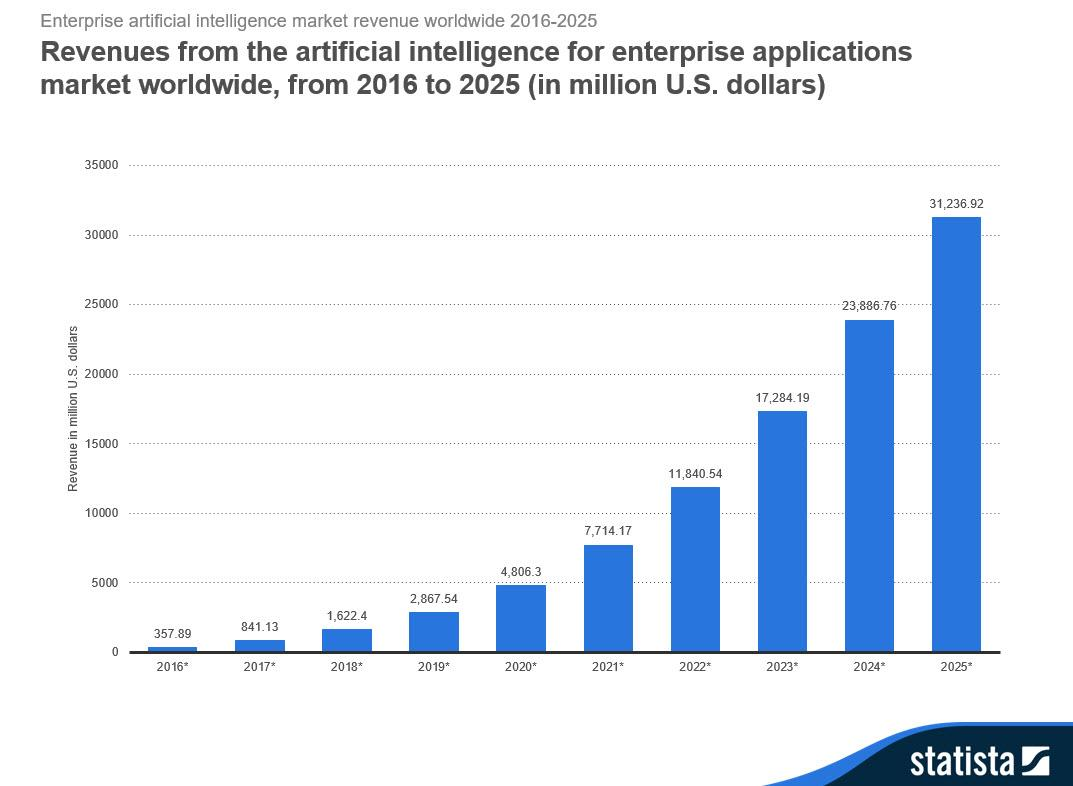
\includegraphics[width=\textwidth]{figures/ai-projections.jpg}
       \caption{Enterprise AI market revenue 2016-2025 (image from \cite{ai-proj}).}
       \label{fig:ai-proj}
   \end{subfigure}%
   ~
   \begin{subfigure}[b]{0.5\textwidth}
       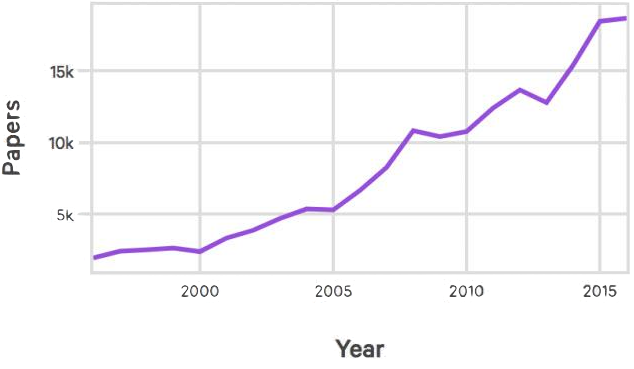
\includegraphics[width=\textwidth]{figures/ai-papers.png}
       \caption{AI papers published per year (image from \cite{ai-papers}).}
       \label{fig:ai-papers}
   \end{subfigure}
\end{figure}

A part of the current EU funding has been allocated to the Human Brain Project (HBP) \cite{hbp}, designated as one of the Horizon 2020 Future and Emerging Technologies Flagship projects with over a billion euros in budget. It is a 10-year initiative launched in 2013 that strives to accelerate the fields of neuroscience, brain-related medicine and computing. The project is broken down into multiple topics, referred to as pillars, one of which is focused on neuromorphic computing to build a novel platform to run neural network simulations. There has never been a unique way of building intelligent systems, and neuromorphic computing is the approach that tries to mimic the morphology of the brain to design hardware in the hope that it will yield the most faithful neural simulations. In the context of HBP, this meant building a novel type of computer with a design directly inspired from the brain which led to the Spiking Neural Network Architecture (SpiNNaker) machine\cite{SpiNNaker-Project}. Spiking neural networks are the neuromorphic version of the traditional artificial neural networks. The latter are "simply" mathematical models trying to approximate the state of the brain, while spiking neural networks will try to reproduce the exact interactions between each brain cell in the hope of getting an even closer approximation. \\

The deliverables of SpiNNaker include a new physical machine, formed of a cluster of neuromorphic printed circuit boards accessible via an online interface for researchers to remotely use. The development process of the machine was iterative, with a single circuit board produced at first which then got assembled in a cluster. For this project, we were fortunate enough to use the first release of the machine: the \textit{102} machine formed of a single circuit board - see Fig.~\ref{fig:spinn3}. The name \textit{102} comes from the machine having approximately $10^2$ cores (72 in fact). The last version of the machine called \textit{106}, meaning it has $10^6 = 1$M cores and there is currently a single version of it (half-finished but functional) at the University of Manchester, where it was built. \\

\begin{figure}[!ht]
   \centering
       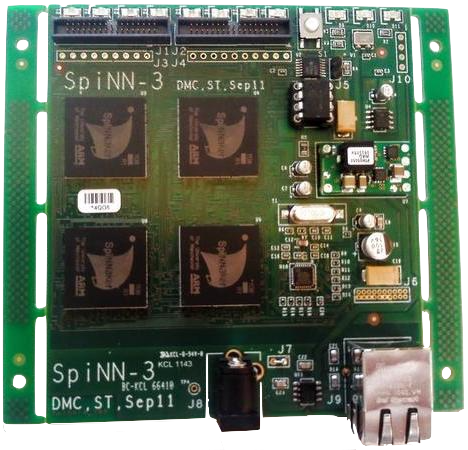
\includegraphics[width=0.7\textwidth]{figures/spin3.png}
       \caption{The SpiNNaker \textit{102} machine, used for prototyping this project (image from \cite{spinn-3}).}
       \label{fig:spinn3}
\end{figure}

These machines present the following hardware characteristics that motivated this project, some of which differ from a classic supercomputer architecture:

\begin{itemize}
\item \textbf{Manycore architecture}: as explained above, the density of cores on the board isthe main design feature inspired from the brain, which has around 86 billions of neural cells \cite{5th-summit}.

\item \textbf{Communication model}: cores communicate through message passing, with messages being small datagrams sent over UDP/IP (72 bits maximum) \cite{ws6}. UDP/IP is a best-effort communication protocol and thus, the sender does not get any guaranty its messages were delivered. This design decision is at the heart of the network layer and is directly inspired from the brain, where a neuron does not get any reception acknowledgement when communicating with neighbouring neurons.

\item \textbf{Communication throughput}: the expected benefit, gained from reducing the message size, was that a greater number of messages could be processed in a second. For cores on the same circuit board, their link can transfer up to 250M bit/s, meaning it could process up to 3M packet/s \cite{ws6}.
\end{itemize}

The details of these hardware specificities will be covered in greater details in the background (section \ref{sec:bg}) of this report. \\

The deliverables of SpiNNaker also include a constellation of specialised software modules that each fulfill a specific mission. Indeed, SpiNNaker is not a regular computer on which users could simply install a Linux distribution and log in. A host machine, connected by Ethernet to SpiNNAker, is needed and pre-compiled binaries can be loaded on selected cores of SpiNNaker from it. This segregation between host and SpiNNaker machine increases the number of software modules needed, which we will cover in greater details in section \ref{sec:sw}. \\

All in all, a SpiNNaker machine can be viewed as a small supercomputer where cores can exchange a considerable amount of small packets at the cost of message delivery reliability. These biology-inspired properties are well suited for spiking neural networks simulations, and illustrate what a neuromorphic computer has the potential to be. It is also these properties that created an opportunity for this project, which we discuss in the next paragraph. \\


\subsection{Objectives}

In order to explore the new opportunities offered by SpiNNaker, we first define the mission statement of this project as follows:

\begin{quote}
\textit{Investigate how we could leverage SpiNNaker for graph processing, using Page Rank as a benchmark, in the hope that it will give a better scalability potential than traditional computers.
}\end{quote}

This project aims to make a contribution to the existing SpiNNaker research by exposing a new application for the machine, since Page Rank has never been ported to the machine before, or at least it never resulted in a publication. Still, alternative applications have already been explored, such as heat equation solving \cite{heat} or Markov Chain Monte Carlo Simulations \cite{markov-on-spinn}, and drawing comparisons with these examples will be interesting in the next sections (\ref{sec:aa}). \\

The reason why graph processing and Page Rank were chosen comes from the data flow of these algorithms.  Indeed, SpiNNaker is optimised for many small-payload exchanges and a single iteration of Page Rank needs to send as many updates as there are edges in its graph. At each iteration, each node sends its weighted rank along its outgoing edges and builds up a new rank by summing the ranks coming from its inbound edges. In SpiNNaker, each of these ranks could be sent as the 32 bits payload of the 72 bits datagram mentioned above. \\

Let us take the concrete example of the Wikipedia page dumps, which are often used as a dataset to bencharmark Page Rank computations. Using the statistics of this study \cite{nayuki} on a dump from early 2014, a graph of all Wikipedia pages was constituted, made of 10M pages (vertices) and 320M links between them (edges). Assuming ranks are encoded with 32 bits, this means at each Page Rank iteration we would need the nodes to exchange $320$M$ \times  32 $bits $= 10$Gb of data. This amount of data could still fit on a single RAM and the computations might not need to be distributed, but for bigger graphs, such as the internet graph indexed by Google, distributing the computation becomes unavoidable. Google claims it has indexed hundreds of billions of pages \cite{google-si} with even more links interconnecting them. This type of graph would require the computation to run in parallel on multiple machines, and the computation being not CPU intensive, the bottleneck probably lies with the communication cost associated with exchanging ranks at each iteration step. To cope with this problem, the biggest edge of SpiNNaker is its low latency interconnect, which would outperform the end-to-end latency of a classic link between two commodity hardware in a data centre. \\

%such as the graph of all Facebook active users, distributing the computations becomes unavoidable. In a dataset from 2011, Facebook had approximatively 721 million users (nodes) for 69 billion friendship links (edges) \cite{fb}. Using the same logic as before, this means the data exchanged per iteration would weigh $69$B$ \times  32 $bits $= 2.2$Tb, and this amount today with Facebook's 2.2 billion active would be even greater \cite{fb-ac-users}.

Consequently, a property we can use to identify algorithms that could scale better on SpiNNaker is the data flow during the computation. If a computation can easily be broken down into \textit{independent} chunks, than this is probably a job more tailored for Map-Reduce \cite{mr}. However, if this is not the case and a lot of state is maintained throughout the computation, with that state needing to be \textit{shared} amongst a lot of workers, than SpiNNaker might be a good alternative. This property is exactly what Page Rank exhibits, and what made it a good choice for a benchmark to confirm this hypothesis about expected improved scalability. \\


\subsection{Contributions}

The contributions from this project are twofold:

\begin{itemize}
\item \textbf{Page Rank simulation framework}: we built the right set of tools to let users run Page Rank simulations effortlessly. Indeed, the software stack of SpiNNaker is quite complex and before implementing anything, a lot of time had to be invested into understanding the SpiNNaker paradigm. These challenges include dependency management of the software modules used, graph vertices mapping to cores, resource allocation, inter-core data routing, algorithm synchronisation barriers between each iteration, resilience to lost packets, results validation and visualisation. All of this complexity is hidden by the framework, and only a list of edges is necessary to quick start a simulation. Details in section \ref{sec:impl}.

\item \textbf{Page Rank scaling}: we demonstrate that Page Rank under SpiNNaker offers better scalability opportunities compared to a traditional PC. We benchmark two implementations of Page Rank: the first one is an (adapted) Python implementation of the well-established \textit{networkx} \cite{networkx} library and second one is a port to SpiNNaker using the framework mentioned above. The performance gain observed shows SpiNNaker allows for a speed-up of a factor of nearly 4 compared to the traditional PC implementation. Details in section \ref{sec:eval}.
\end{itemize}


Here, Page Rank is used as a proof-of-concept but this project aims to show that an entire class of algorithms are well suited for a port to SpiNNaker. The framework provided can easily be extended to support other graph-based algorithm with a data flow similar to Page Rank.

\newpage
\section{Background} \label{sec:bg}

This project investigates the potential of SpiNNaker on alternative applications, so this background section will provide the reader with a thorough understanding of neuromorphic computing and how it gave birth to SpiNNaker (section \ref{sec:nmc}). Then, we will focus on the specification of the SpiNNaker machine, from its hardware properties to the existing software stack that lets us harness its potential (section \ref{sec:smc}). Finally, we will review how the machine can be used to run spiking neural network simulations, which was the goal application of their designers. We will also see how alternative applications have been exploring the potential of SpiNNaker and use it as an inspiration for our own implementation of Page Rank (section \ref{sec:usage}).

\subsection{Neuromorphic computing} \label{sec:nmc}

\subsubsection{History}

Neuromorphic computing is a young field that is considered to have been pioneered by Dr. Carver Mead, an American scientist and engineer who is currently a Professor Emeritus at the University of California \cite{mead}. In 1988, he co-authored a paper in which he explained how he built the first analog model of a retina on a silicon chip \cite{retina}. By mimicking the biological behaviour of a retina on a circuit board, Mead introduced a new class of hardware that would become a field of computing of its own: neuromorphic computing. \\

Interestingly, this recent focus would not only have been prompted by the need for more accurate neural simulations, but also by the long-predicted end of Moore's Law. These considerations are well summarised by the following excerpt of an article from the Association for Computing Machinery (ACM): \textit{As the long-predicted end of Moore's Law seems ever more imminent, researchers around the globe are seriously evaluating a profoundly different approach to large-scale computing inspired by biological principles. In the traditional von Neumann architecture, a powerful logic core (or several in parallel) operates sequentially on data fetched from memory. In contrast, \textit{neuromorphic} computing distributes both computation and memory among an enormous number of relatively primitive \textit{neurons}, each communicating with hundreds or thousands of other neurons through \textit{synapses}. Ongoing projects are exploring this architecture at a vastly larger scale than ever before, rivaling mammalian nervous systems, and developing programming environments that take advantage of them} \cite{acm}. \\

In 2013, one probably precipitating the other, two large initiatives were launched in the US and in Europe aiming to revolutionise our understanding of the human brain \cite{theeco}. All simulations thus far were ran on small networks of the brain, and people started to believe we needed to simulate significant chunks of the brain to be able to map higher-level processes, such as consciousness. We just did not have the right tools to study the brain, so they had to be built. On the American side, the BRAIN initiative was started by the Obama administration in April 2013 \cite{brain} and led to DARPA's SyNAPSE board built from IBM's TrueNorth chips a year later. Each of these neuromorphic chip can simulate over a million neurons and 268 million programmable synapses \cite{truenorth} that are used to unveil the mysteries of the human brain. \\

\subsubsection{Human Brain Project} \label{sec:hbp}

On the European side, the Human Brain Project (HBP) was launched with a spectacular projected cost of 1.3 billion euros and designated as a Future and Emerging Technology (FET) Flagship project. The amount of resources invested illustrate well the importance of the project, and the high expectations the Europeans placed in it. Part of the goal of this project was to create an advanced neuromorphic computing platform featuring two state-of-the-art biology-inspired supercomputers \cite{nmp} \cite{ncp}. These two machines are the BrainScaleS located in Heidelberg University, Germany (Fig.~\ref{fig:brainscales}) and the SpiNNaker 106 machine at the University of Manchester, United Kingdom (Fig.~\ref{fig:spinnaker106}).

\begin{figure}[!ht]
    \centering
    \begin{subfigure}[b]{0.47\textwidth}
        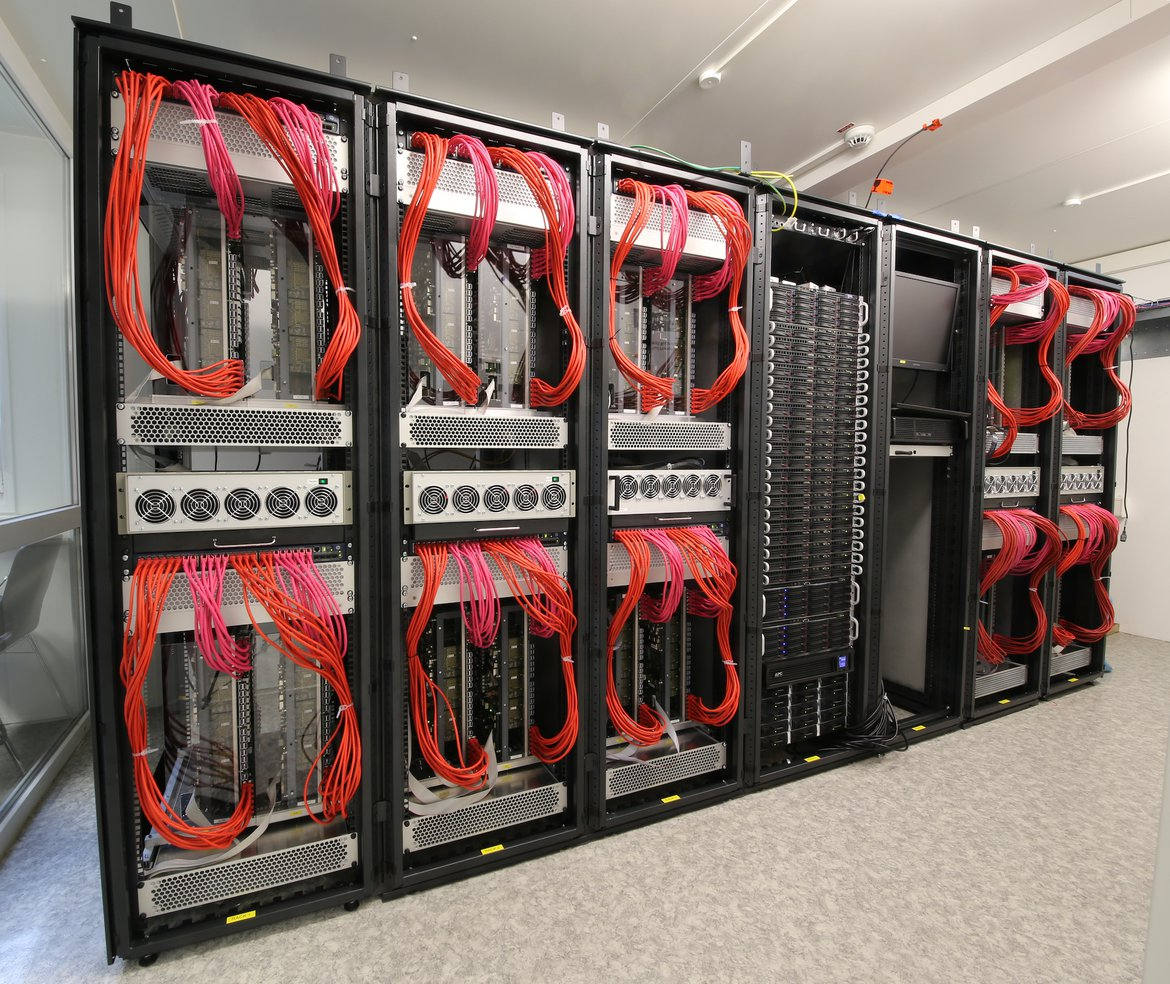
\includegraphics[width=\textwidth]{figures/brainscales.jpg}
        \caption{BrainScaleS supercomputer (image from \cite{nmp}).}
        \label{fig:brainscales}
    \end{subfigure}%
    ~
    \begin{subfigure}[b]{0.53\textwidth}
        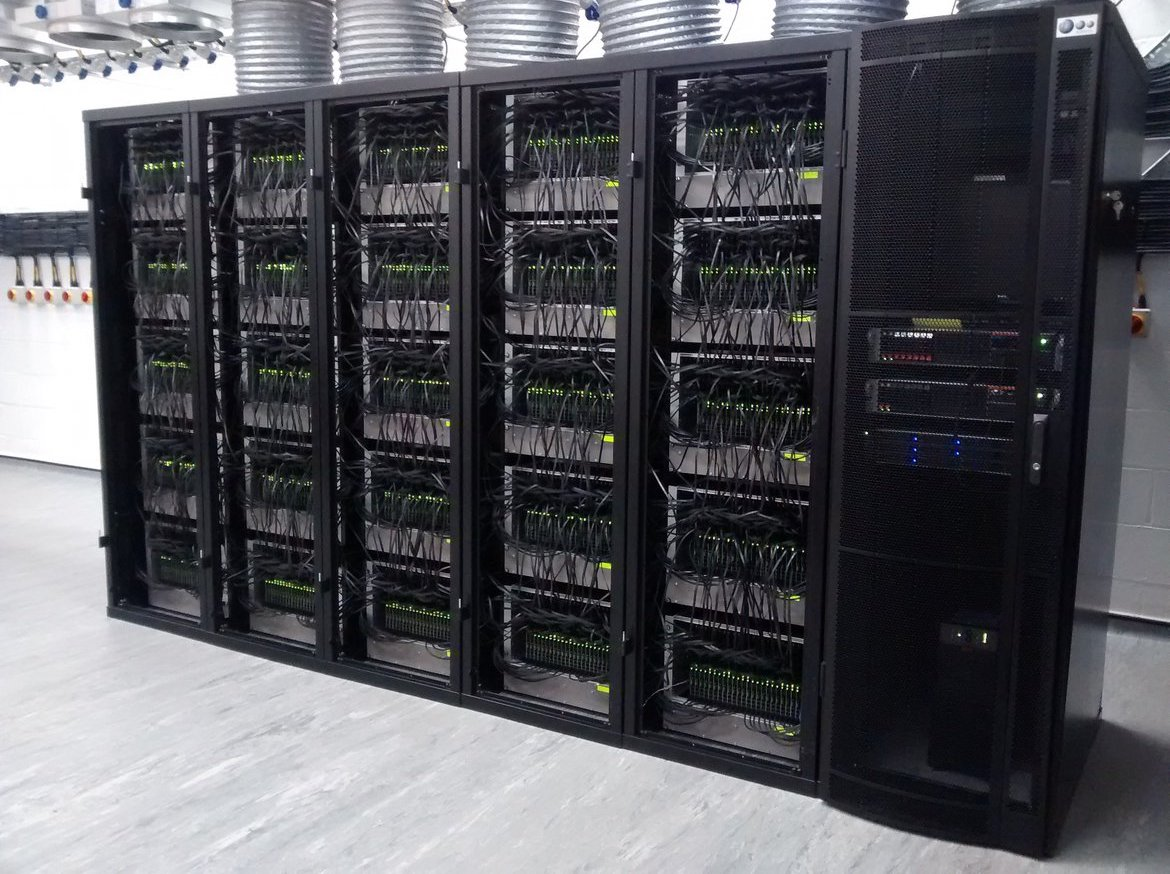
\includegraphics[width=\textwidth]{figures/spinnaker106.jpg}
        \caption{SpiNNaker supercomputer (image from \cite{nmp}).}
        \label{fig:spinnaker106}
    \end{subfigure}
\end{figure} 

These two machines explore two different approaches to building a neuromorphic silicon brain. The BrainScaleS system is arguably the most neuromorphic approach, as it is based on the physical emulation of neurons using analogue and mixed-signals. Thus, there is no source code that the machine would execute step by step as in a von Neumann architecture computer. Rather, the system evolves according to the physical properties of the machine, running ten thousand times faster than a human brain would \cite{hw}. This means a day worth of real human brain training can be compacted in slightly over a minute, which drastically speeds up the workflow of neuroscientists experimenting with the machine. On a similar topic, it also seems noteworthy to mention Intel's Loihi \cite{loihi}, the state-of-the-art neuromorphic chip released in 2018, using an approach comparable to BrainScaleS, and that claims to outperform all existing hardware in its field. \\

Although this approach is faithful to the biology and is extremely energy efficient, it implements a fixed neuronal and synaptic model which restricts model exploration. This is why a second approach was taken with SpiNNaker, a neuromorphic computer of another kind where any neuronal and synaptic model could be implemented. As we use this machine for the project, we dedicate the next section to covering it in greater details. \\

\subsubsection{SpiNNaker}

Although the Human Brain Project \cite{hbp} was launched in 2013 with the EU funding, the SpiNNaker project had already started back in 2005. At the time, it was backed by the \textit{Engineering and Physical Sciences Research Council} (EPSRC), the main agency funding research initiatives in engineering and physics in the United Kingdom (UK). \\

\paragraph{Spin1 - test chip}

Working closely with neuroscientists, researchers from multiple UK universities spent years designing and experimenting to be able to deliver Spin1 in 2009, the SpiNNaker test chip Printed Circuit Board (PCB) \cite{dev-process}. It was intended as a proof of concept to demonstrate the design of the chip worked, and featured the first 4 SpiNNaker chips containing 2 ARM968 cores each. It was also formed of the common features that can be found on a PCB: power supply, LEDs, Ethernet interface as the primary communication channel with the host machine, SpiNNaker Link Connectors to chain multiple boards, extra testing facilities; see Fig.~\ref{fig:spin1} \\

\begin{figure}[!ht]
\centering
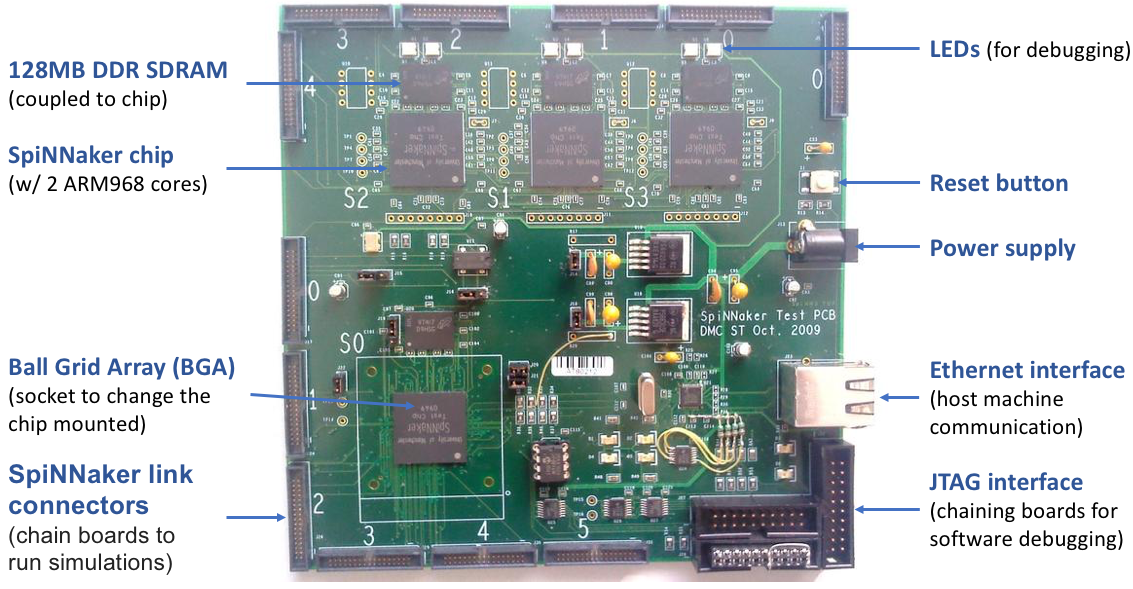
\includegraphics[width=\textwidth]{figures/spin1-schema.png}
\caption{Architectural schema of the Spin1 test chip PCB (image adapted from \cite{dev-process})}
\label{fig:spin1}
\end{figure} 


\paragraph{The challenge of power consumption}

Part of these testing facilities measured the energy consumption of the board. As a matter of fact, we know the human brain uses less than 20W to function so it was identified as a primary goal to build a PCB as energy-efficient as possible, even at the cost of some performance tradeoffs. Indeed, we are still far from properly understanding how the human brain works, but the knowledge we have of it has already taught us three lessons for building brain-inspired computers: massive parallelism, resilience to component failure and finally, energy-efficiency \citep{bic}. The latter was achieved at two complimentary layers:

\begin{itemize}
\item \textbf{Hardware}: the choice of the harware, and in particular of the ARM968 cores, was driven by energy efficiency. This is confirmed by the technical reference manual of the processor: \textit{the ARM968E-S processor is targeted at a wide range of embedded applications that require high performance, low system cost, small die size, and low power.} \cite{arm968} This class of processor takes low power usage as a compulsory requirement, and then tries to maximise the performance it can get out of the processor. Indeed, this core only runs at 200-MHz, which is an order of magnitude below the speed of a commodity PC processor. They typically power embeded devices, such as smartphones, and let the entire million-core machine run with at most 75 kW of electrical power during peaks \cite{spinnaker}. % Maybe say something about 1200*75 = 90kW !

\item \textbf{Software}: the programming model of the SpiNNaker Application Programming Interface (API) is event-driven. This paradigm allows the cores to be kept in a low-power state when they are not handling any events, which is not the case for the typical retail CPU. The ultimate goal of systems like SpiNNaker would be to achieve energy-proportional computing \cite{energy-prop}, where an idle core would not consume any power and where power usage would be proportional to the compute load of the core. As a mean of comparison, for a typical CPU in a data centre today, the power consumption is only divided by half when going from a full compute load core to an idle core, see Fig.~\ref{fig:energy-non-prop}. It would be interesting to see how far is SpiNNaker from being an energy-proportional computer, the benchmarks do not seem to have been published.
\end{itemize}
 
\begin{figure}[!ht]
\centering
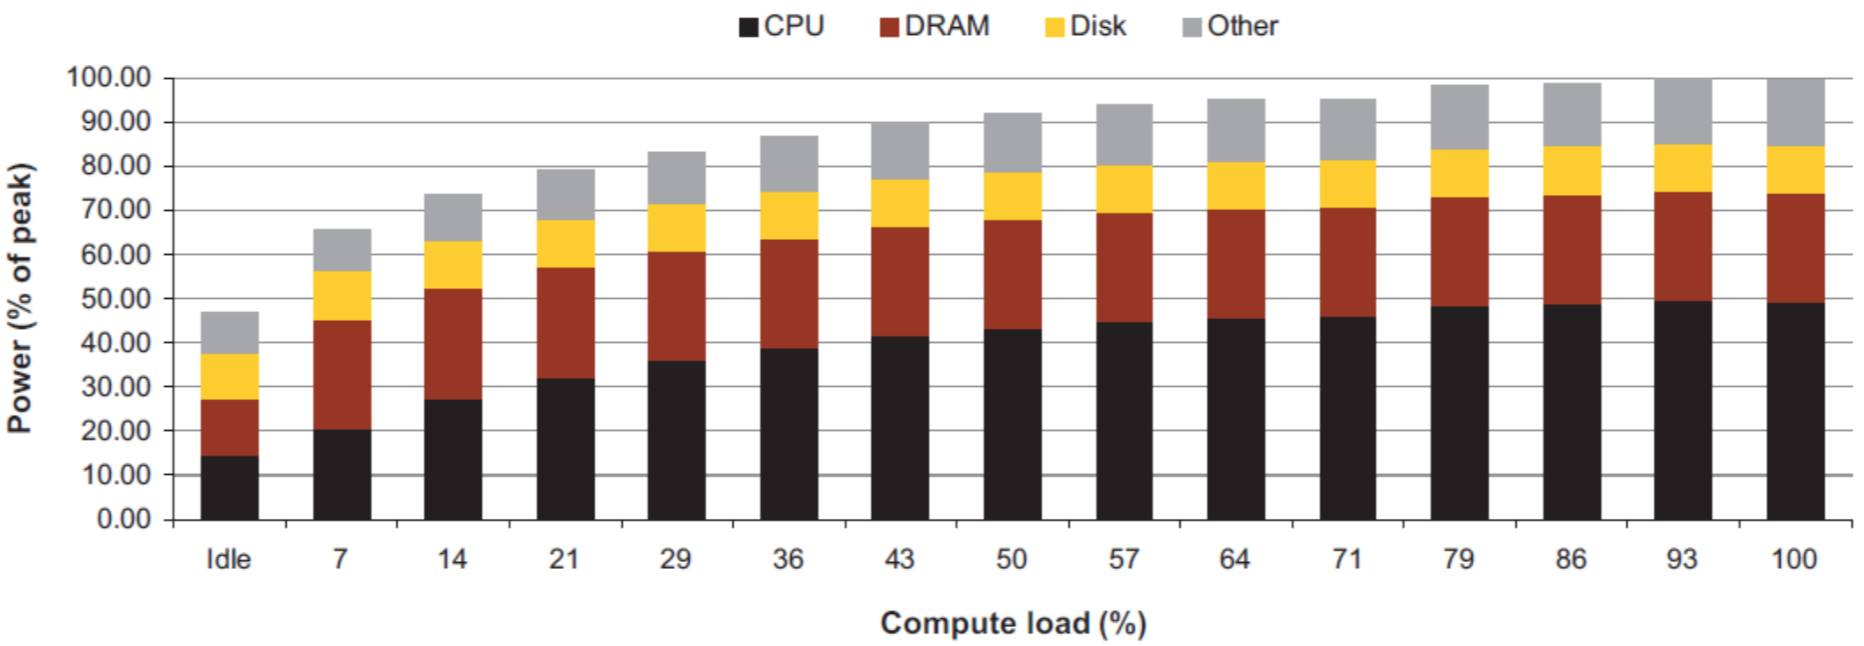
\includegraphics[width = 1\hsize]{figures/energy-non-prop.png}
\caption{Power consumption of a typical datacentre CPU (image from \cite{energy-non-prop}).}
\label{fig:energy-non-prop}
\end{figure}


\paragraph{Spin2 - production chip test}
 
After the success of the first Spin1 board, this new release from 2011 was mainly aimed at scaling \textit{up} the design. Each SpiNNaker chip would now embed 18 ARM968 cores instead of the 2 in the previous model. Moreover, the mobile Double Data Rate (DDR) Synchronous Dynamic Random-Acess Memory (SDRAM) was now embedded in the SpiNNaker chip package. Indeed, each chip has its own shared memory slot for all its cores to use. Additionally, a USB interface was added to allow the board to be reset remotely without having the press the physical button on the board. Finally, some of the extra elements used for testing in Spin1 (e.g. for power consumption) were removed as the board had already passed some of these tests; see Fig.~\ref{fig:spin2}.


\begin{figure}[!ht]
\centering
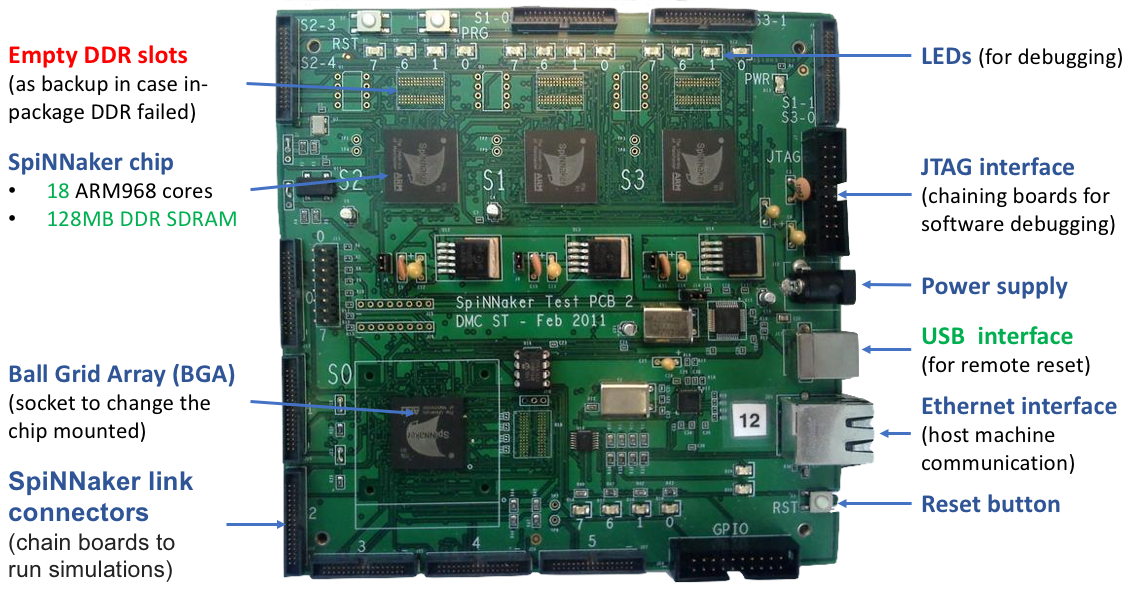
\includegraphics[width=\textwidth]{figures/spin2-schema.png}
\caption{Differential architectural schema of the Spin2 production chip test PCB, illustrating the design updated from Spin1 (image adapted from \cite{dev-process}).}
\label{fig:spin2}
\end{figure} 

\newpage
\vspace*{-1.2cm}
\paragraph{Spin3 - general purpose PCB}

Later in 2011, Spin3 was released after a few minor modifications to Spin2. The novelty of the board was to be general purpose, which made it the first usable SpiNNaker neuromorphic PCB for the research community. The surface of the board was also reduced by a factor of three, from $15 \times 15 = 225cm^2$ down to $8 \times 9 = 72cm^2$, to make it possible to fit it on a small robot. The design also got rid of all the hardware support for testing: BGA socket, power consumption monitoring, USB interface, reduced JTAG interface, reduced LED support per chip. Additionally, the number of SpiNNaker link connectors was also brought down to 2 as this board was not intended for large clusters of connected boards but rather for prototyping; see Fig.~\ref{fig:spin3}.

\begin{figure}[!ht]
\centering
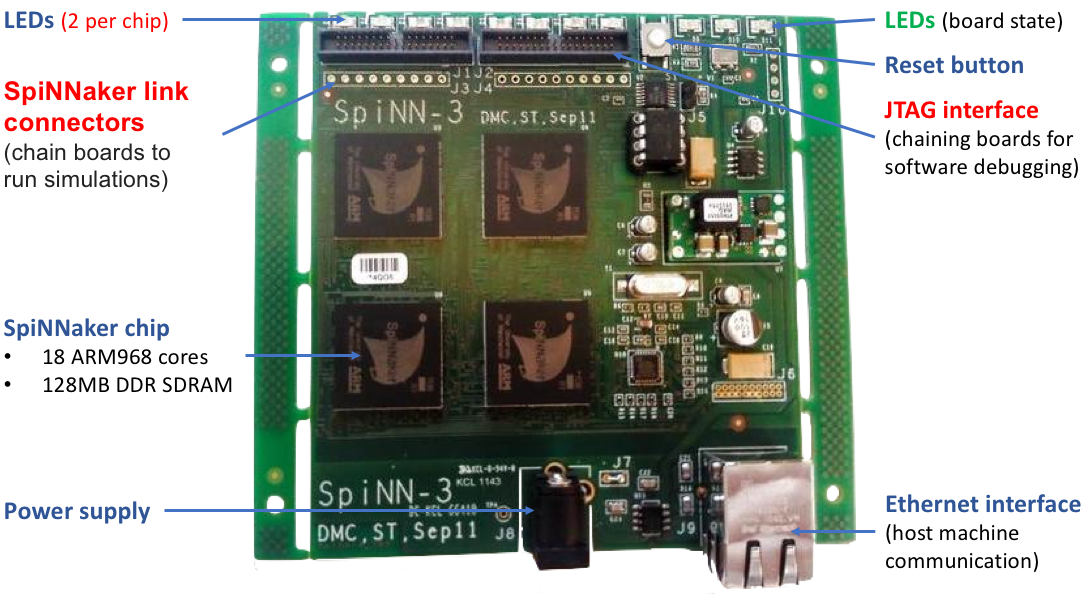
\includegraphics[width=\textwidth]{figures/spin3-schema.png}
\caption{Differential architectural schema of the Spin3 general purpose PCB, illustrating the design updated from Spin2 (image adapted from \cite{dev-process}).}
\label{fig:spin3}
\end{figure} 


\newpage
\paragraph{Spin4 - 48 chips PCB}

\begin{wrapfigure}{r}{0.4\textwidth}
  \begin{center}
    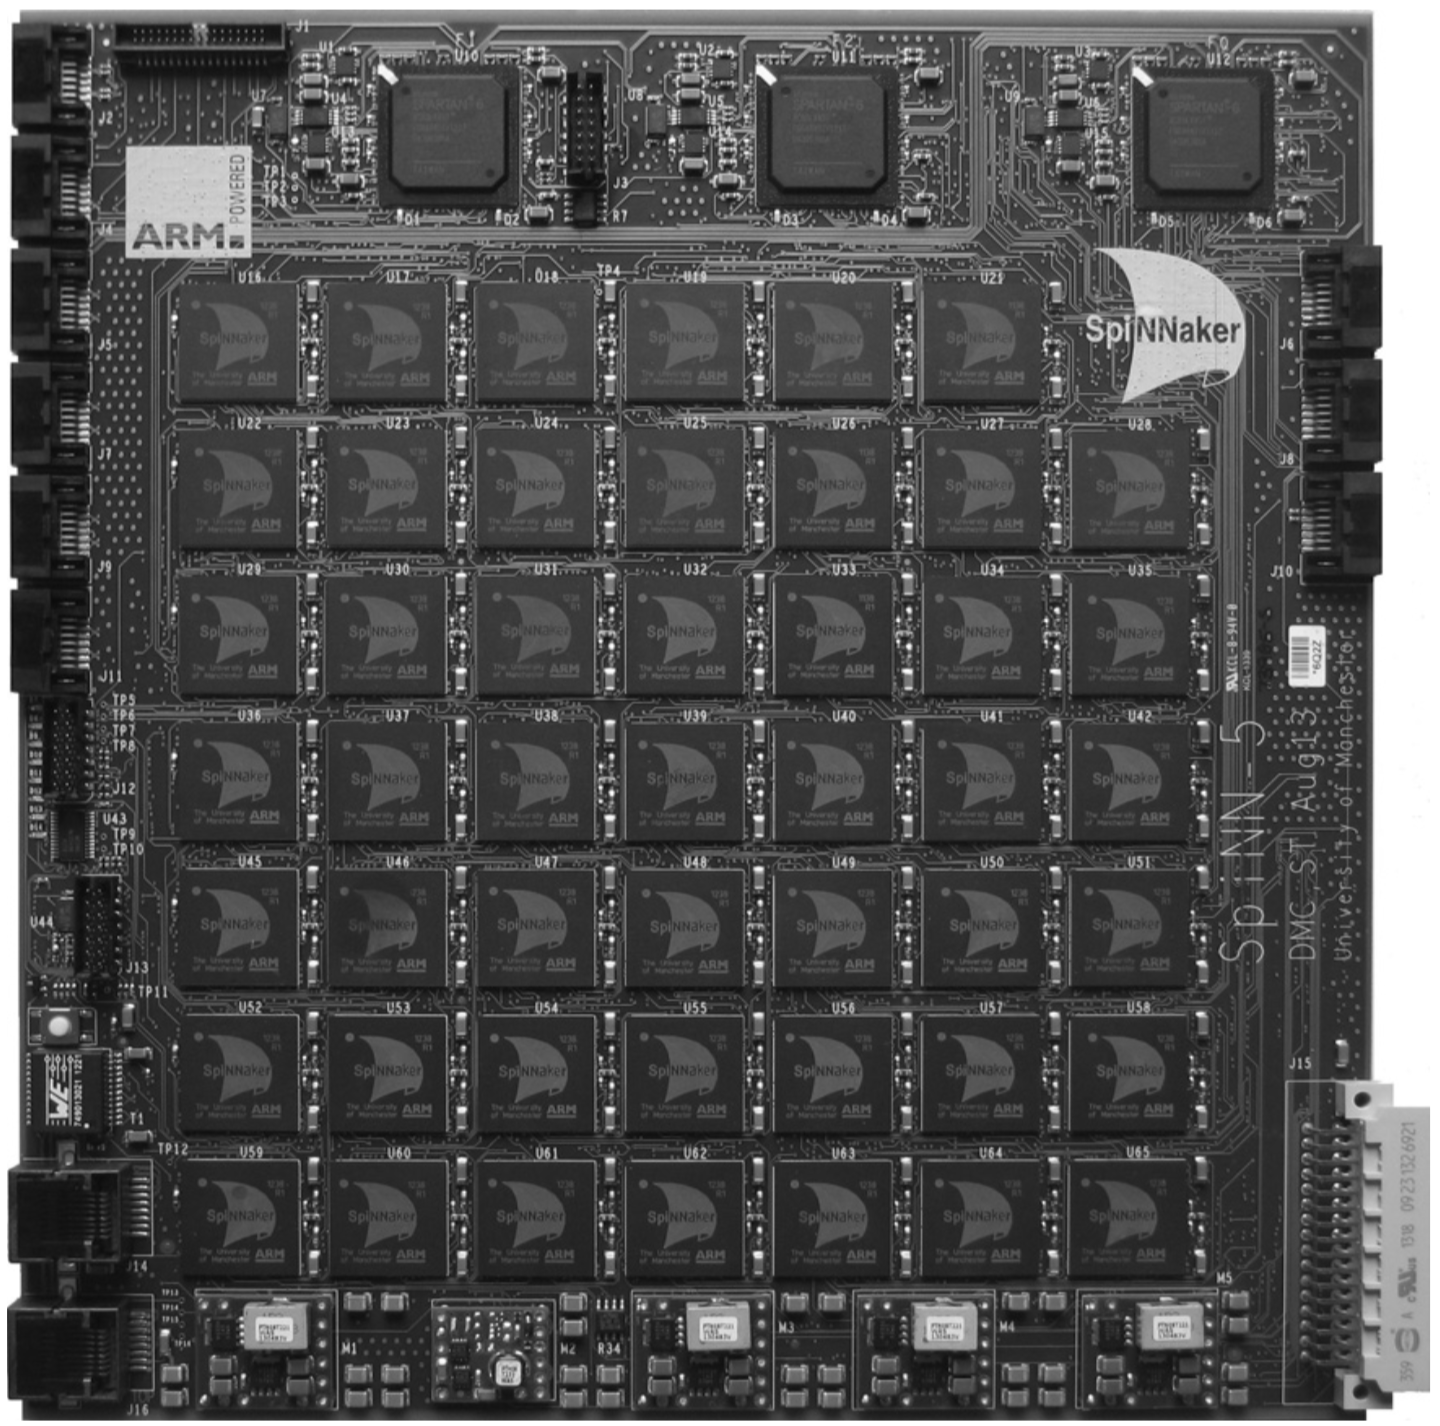
\includegraphics[width=0.38\textwidth]{figures/spin4.png}
  \end{center}
  \caption{The Spin4 PCB with 48 chips (image from \cite{bic}).}
  \label{fig:spin4}
\end{wrapfigure}

Finally, an ultimate version of the board was made to scale \textit{out} the previous design. At this stage, SpiNNaker chips had demonstrated they were functional so the main focus was to fit 48 chips on the same board. As a matter of fact, the ultimate goal of the project was to combine 1200 such boards and doing so would result in the million-core neuromorphic computer targeted. Indeed, $1200 \times 48 \textnormal{ chips } \times  18 \textnormal{ cores } \approx 1M \textnormal{ cores}$ and each core is expected to simulate a thousand neurons, which gives the expected one billion neurons real time simulation (and one million neurons per Spin4 PCB, see Fig.~\ref{fig:spin4}). As of today, the University of Manchester runs the largest version of the SpiNNaker machine with 500K cores, although they plan on expanding it over the coming months to reach the million of cores \cite{act-project-access}. \\ % TODO: don't we say they have a million somewhere? 
 
Regarding power usage, the peak consumption of the Spin4 board was of 75W for a real time simulation of a million neurons \cite{dev-process}. As a comparison, IBM's TrueNorth chip, which has a design closer of BrainScaleS than SpiNNaker, is able to simulate one million neurons as well but only consumes 65mW of power while running a typical computer vision problem \cite{truenorthpaper}. But as BrainScaleS, TrueNorth has a physical model approach (see section \ref{sec:hbp}) so the power consumption comparison is probably unfair. Comparing SpiNNaker with the Sunway TaihuLight in China is probably fairer. It is now the second biggest supercomputer in the world (after newly released Summit stole the title on June 8th 2018 \cite{summit}) and number 20 on the GREEN500 list (top 500 supercomputers ranked by energy efficiency) \cite{green500}. The Sunway TaihuLight has 10,649,600 cores running at 1.45GHz for a power consumption of 15,371 kW \cite{top500} while SpiNNaker has 1,036,800 cores running at 0.2GHz for a power consumption of 75kW \cite{spinnaker}. By using an (approximative) performance per watt measure (usually in FLOPS/watts), we compute the ratio of the computer power (in GHz) over the power consumption (in kW), we find SpiNNaker more energy efficient by factor of 2.8:

\vspace*{-0.3cm}
\begin{equation*}
\begin{split}
R_{SpiNNaker} &= \frac{1,036,800 \times 0.2}{75} \\
R_{TaihuLight} &= \frac{10,649,600 \times 1.45}{15,371} \\
\frac{R_{SpiNNaker}}{R_{TaihuLight}} &\approx 2.8
\end{split}
\end{equation*}

However, computing the same ratio against the top GREEN500 computer, the Shoubu system B \cite{green500}, places SpiNNaker 7 times less energy efficient. Consequently, SpiNNaker probably does not defeat to current GREEN500 podium, but still achieves a very good energy efficiency that rivals with the state-of-the-art supercomputers in that matter. \\

Now that we have clearly described the hardware we will be using (the Spin3 board for the prototyping phase), let us now focus on how the internals of the machine actually work and interact.

% previous was "what we have", now is "how it works"
\subsection{SpiNNaker machine characteristics} \label{sec:smc}

First in section \ref{sec:hw}, we will focus on the hardware inside a SpiNNaker chip. Then, we will review in section \ref{sec:nw} the network topology that connects multiple chips together. Next, we will detail the transmission protocol used in that network - section \ref{sec:aa}. Finally in section \ref{sec:sw}, having it mind that physical layer, we will be able to understand what software stack was built on top of it to make the SpiNNaker machine a truly powerful tool.

\subsubsection{Chip architecture} \label{sec:hw}

The piece of hardware at the forefront of the design was the SpiNNaker chip (called a \textit{node} interchangeably), see Fig.~\ref{fig:spinn-core-labeled}. 

\begin{figure}[hbtp]
\centering
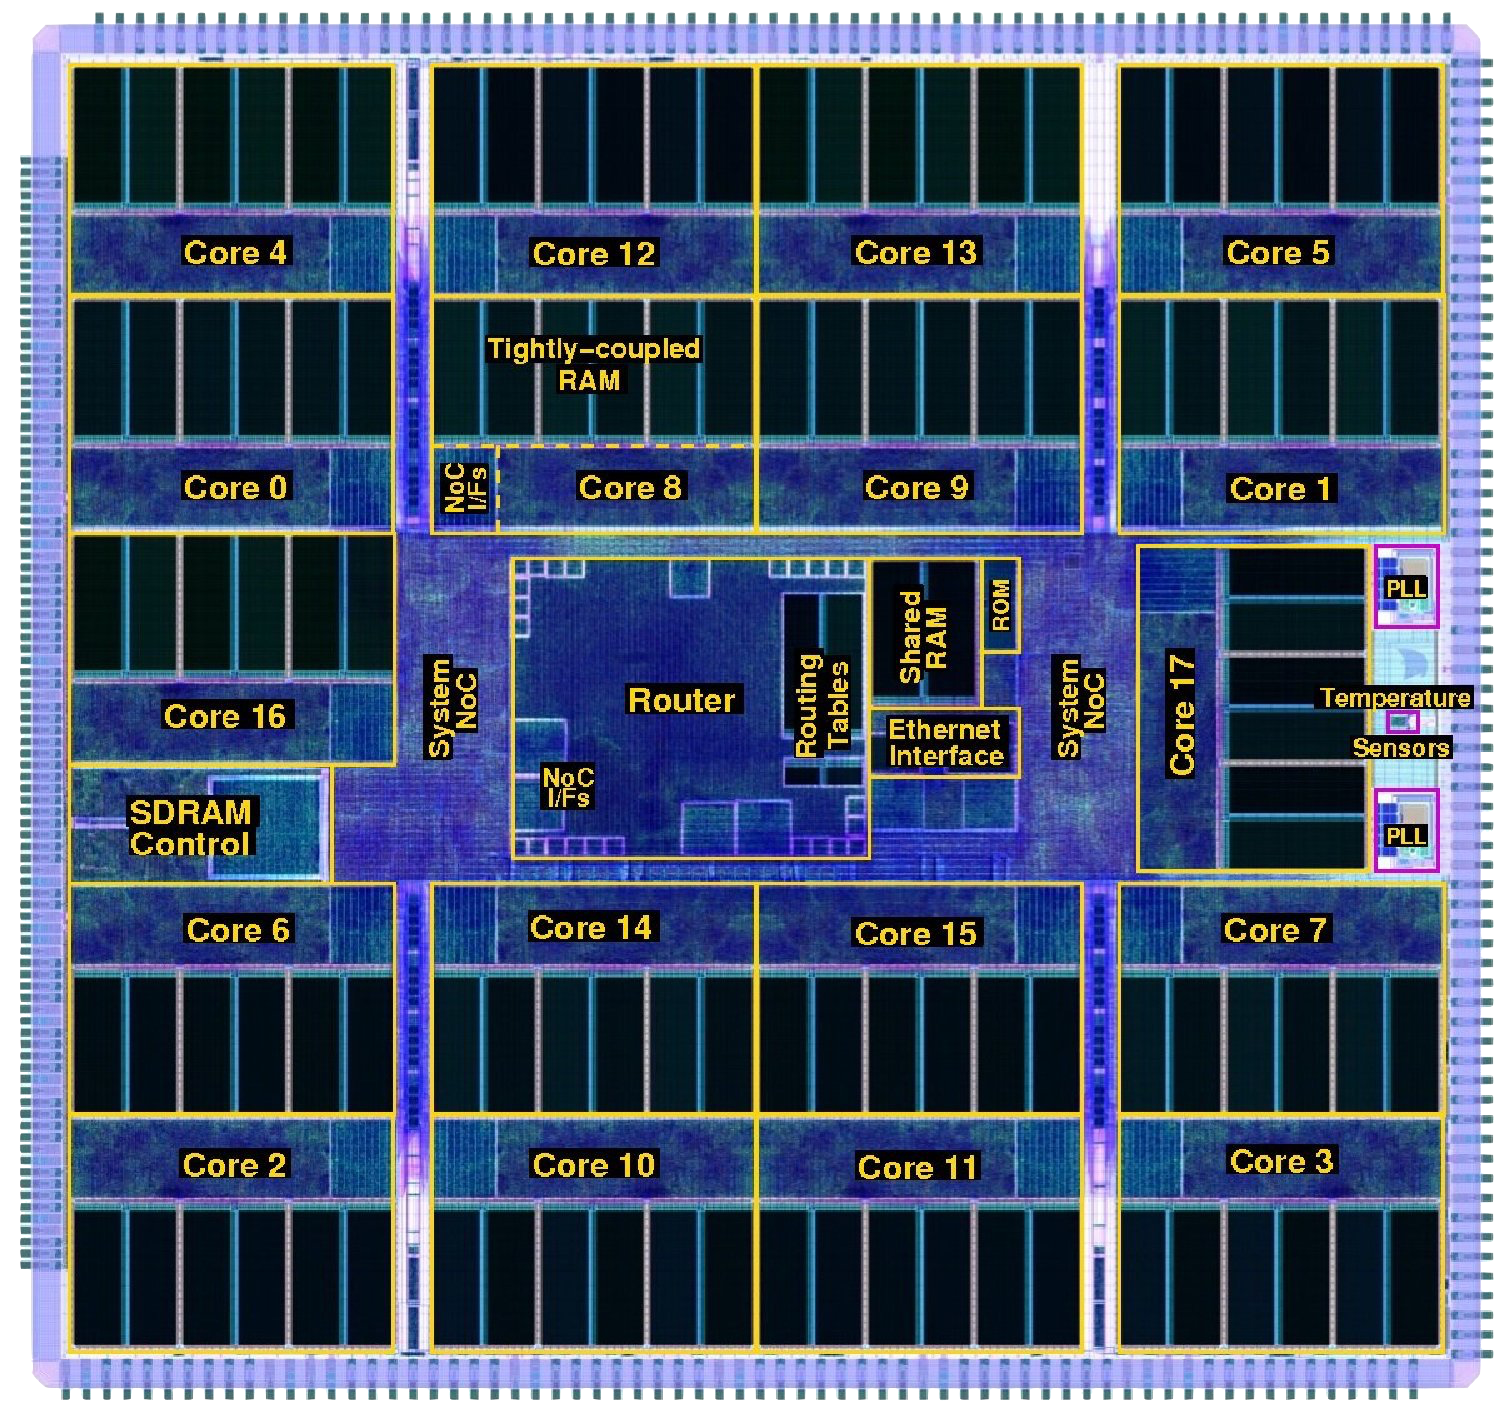
\includegraphics[width = 0.8\hsize]{figures/spinn_labeled_bw.png} 
\caption{The die plot of a SpiNNaker node, with 18 ARM cores (image from \cite{spinn-core}).}
\label{fig:spinn-core-labeled}
\end{figure}

Slides from a 2015 workshop \cite{spin-chip-resources} give an overview of the content of the chip:

\begin{itemize}
\item \textbf{Shared memory}: 128 MB of DDR SDRAM is shared between all the cores of the chip. It is located off-chip, but usually in the same package; hence the SDRAM controller as a on-chip interface to access it. In combination with 32 hardware locks on the chip, they allow powerful abstractions to be implemented, such as semaphores which we will use in the project implementation (detailed in section \ref{sec:prsf}).

\item \textbf{Router}: to forward packets in and out of the chip. Similar to the brain and as opposed to high-performance computers, SpiNNaker cores communicate via a packet-switched network optimised for large numbers of small fixed-sized data packets sent over UDP/IP (\textit{message passing}). Indeed on a regular computer, cores on the same chip usually share L2 or L3 caches and use it as a communication vector to synchronise computations reliably (\textit{shared memory}). To support multicast routing, where a packet sent once can be delivered to multiple destinations, a routing table of 256 associative entries \cite{testchip} can be configured to specify how to route each packet based on its key (detailed in section \ref{sec:nw}). Finally, we can note that using the User Datagram Protocol (UDP), a very simple transfer protocol with no fail-safe, is a deliberate biology-inspired design decision. UDP has no error checking, no packet sequencing and this built-in lack of reliability has led some people to refer to it as the 'Unreliable Datagram Protocol' \cite{udp}. Thus, it is fit to represent neuron-to-neuron interactions that are also based on a best-effort communication scheme.

\item \textbf{NoC}: Asynchronous Network on a Chip (NoC) that unifies the level of abstraction provided by the router, by allowing packets travelling between two cores of the same chip to be treated as any cross-chip communication.

\item \textbf{Cores}: 18 ARM968 cores running at 200MHz with a performance of 220 DMIPS. At boot time, each core will be assigned one role according to the following requirements: 16 application cores, 1 monitoring core and 1 spare core. The applications cores are the ones running the user code and implement a given simulation, such as a spiking neural network. The monitoring core is responsible for coordinating the work of the application cores. For instance, any command that comes from the host machine is targeted to the monitoring core, that will then execute that command on the application cores it manages. Lastly, a spare core is a redundancy added for defect-tolerance, taking here again some inspiration from the brain which looses about 200,000 neurons a day unnoticed \cite{neuron-loss}. 

To equip each core, they all come with a DMA controller, to copy from and to shared memory at a low latency (15ns)\cite{spin-chip-resources} and without a CPU overhead. Additionally, each core comes with a communications controller (to interface with the router) and a vectored interrupt controller (to support the event-driven programming paradigm of SpiNNaker).

\item \textbf{TCM}: Each core also has 96KB of Tightly Coupled random-access Memory (TCM), that is mounted on top of the core to minimise latency (5ns) \cite{spin-chip-resources}. This memory space is partitioned into two dedicated memory subspaces: 32KB of Instruction TCM (ITCM) where the active binary is loaded and 64KB of Data TCM (DTCM) to be freely used by the program running on the core.
\end{itemize}

The following hardware elements are part of the chip internals tools, and are mainly used by the monitor processor (used interchangeably with \textit{core}):

\begin{itemize}
\item \textbf{Ethernet} interface: used for interactions with the host machine. The monitor core is in charge of handling these interactions.

\item \textbf{System ROM}: a 32KB memory space with that is executed on chip start up to boot the system. It first runs a self-test, then starts the monitor processor selection process, bootstraps the router and eventually boots the remaining components of the chip \cite{testchip}.

\item \textbf{System RAM}: a 32KB memory space used primarily by the monitor core to optimise its system operations.

\item \textbf{Sensors}: three sensors to record temperature variations on the chip; remainders from the testing stages of the chip.

\end{itemize}

When the chip starts, the self-test phase of the System ROM will identify all valid cores. For example, if a core is detected to have failed, the algorithm will decide to use the spare core but that will remain invisible to the end user. Indeed, SpiNNaker defines a notion of Virtual Core \cite{vcpu} where each running core has both a physical identifier (hardware core ID) and a virtual identifier (exposed to user). Once the monitor processor selection has ran and chosen a core at random, it returns the physical identifier of this core which is mapped to the Virtual Core 0. Then, up to 16 physical cores are assigned a virtual identifier following an incrementing counter. These virtual identifiers help make the chip resilient to core failures, without exposing any of the hard-coded identifiers that might fail, always returning a list of consecutive and functional cores. This design is similar to hard disk drives, which have a physical mapping of sectors but will only expose a logical mapping of these sectors that factors out bad sectors. \\

After this overview of how a chip works, let us see how multiple chips work together and how data flows through SpiNNaker. 

\subsubsection{Network topology} \label{sec:nw}

The SpiNNaker chips are arranged in a 2D triangular mesh network with bidirectional links to 6 neighbours \cite{testchip}, as show on chip (1,1) in Fig.~\ref{fig:mesh}.

\begin{figure}[hbtp]
\centering
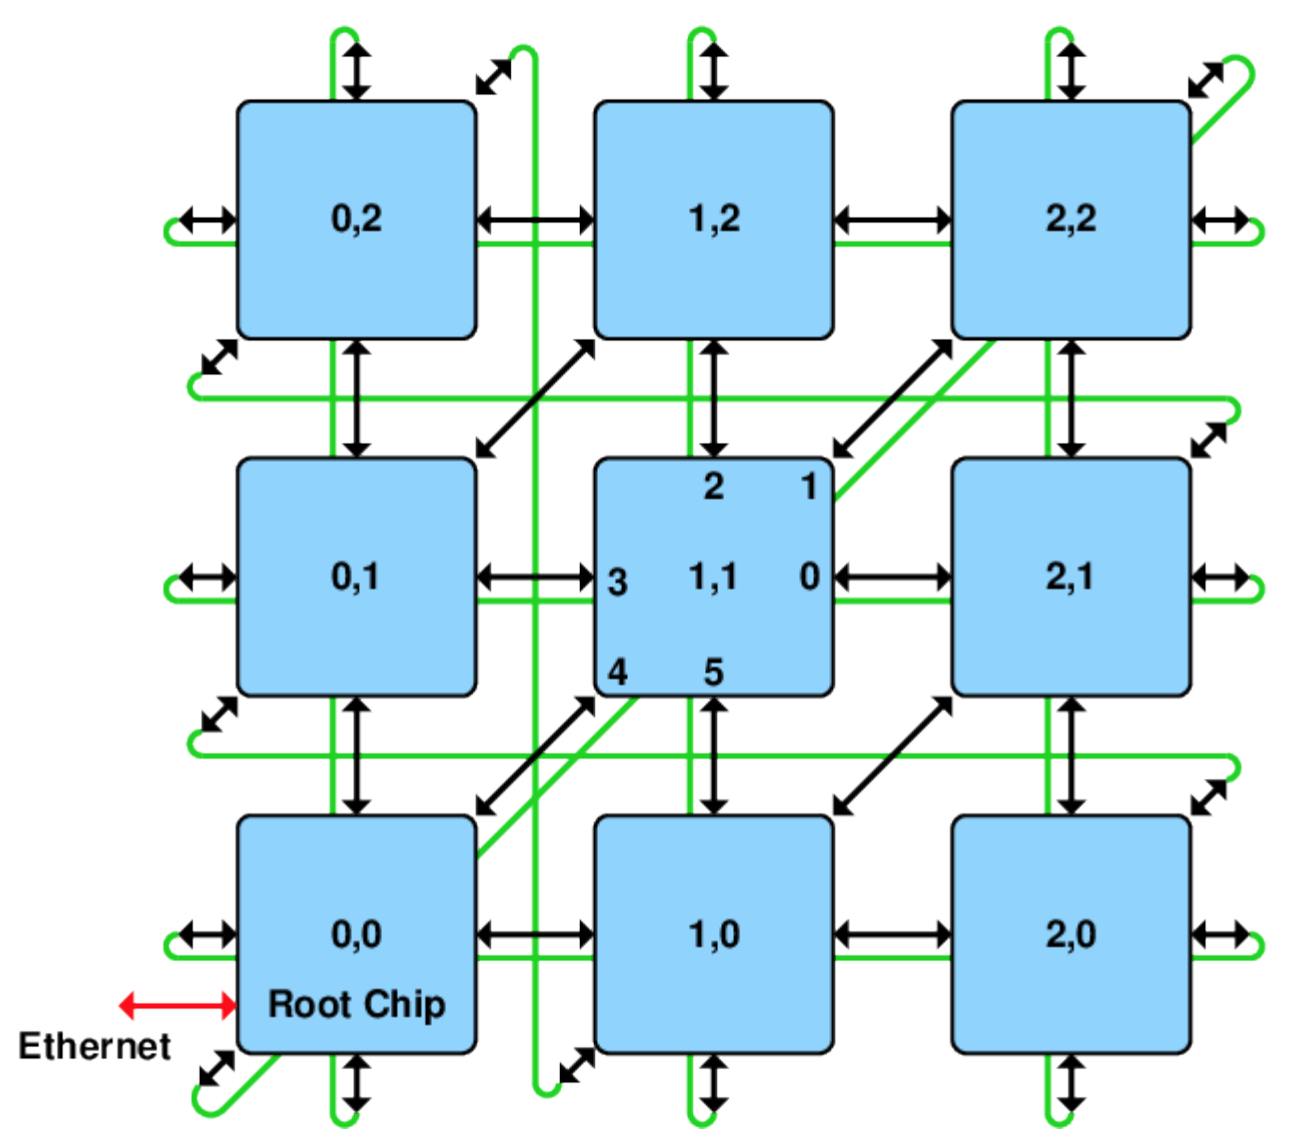
\includegraphics[width = 0.8\hsize]{figures/mesh.png}
\caption{2D mesh network interconnecting SpiNNaker chips (image from \cite{mesh_img}).}
\label{fig:mesh}
\end{figure}

During system bootstrap, a flood-fill discovery mechanism identifies all the chips available and initialises a 2D array of SpiNNaker chips that is exposed to the host machine. The similarity with Virtual Cores is clear, and this logical mapping has the advantage of allowing for dynamically changing network topologies at boot time. The host machine, connected to one of the circuit boards by a 100Mbit/s Ethernet cable, designates the root chip: the chip (0,0) on that connected board. Then, at boot time, the chip will discover the chips around it on the same board, which will in turn discover all the connected boards with their chips. Another advantage of this dynamic topology is defect-tolerance, where a defective chip can simply be removed from the network logical mapping. \\

Now that the network structure is clear, let us see what data flows through it by giving an overview of the transmission protocols used to move data in SpiNNaker. \\


\subsubsection{Data transmission protocols} \label{sec:tp}

\paragraph{Packet format}  \label{sec:pf}

Each core has its own communications controller that is responsible for formatting outbound packets and parsing those incoming. Any SpiNNaker packet will be of either 40bits or 72bits (with a 32bits payload) and will be of one of the following four forms \cite{testchip}:

\begin{itemize}
\item \textbf{Multicast (MC)} packet, sent once and potentially has multiple destinations. Routing is determined by a key given by the sender. 

\textit{Usage}: primary communication format for application cores that propagate neural events to other application cores in the system.

\item \textbf{Point-to-point (P2P)} packet, unicast transmission between a source and a destination core. 

\textit{Usage}: system management, e.g. to load a given executable on a core.

\item \textbf{Nearest-neighbour (NN)} packet, unicast or broadcast transmission with  neighbours. The neighbours are the six directly connected chips, as show on Fig.~\ref{fig:mesh}. For a unicast transmission, the target will be one of these neighbours or the local monitor processor on the chip. For a multicast transmission, the packet will be sent to all six neighbours.

\textit{Usage}: system flood-fill algorithms, e.g. for discovery when bootstrapping the system.

\item \textbf{Fixed-route (FR)} packet, unicast transmission with the host system.

\textit{Usage}: to move debugging data from a core back to the host machine.
\end{itemize}


\paragraph{SpiNNaker Datagram Protocol (SDP)}

For the sake of completeness, we also need to mention the SpiNNaker Datagram Protocol (SDP) \cite{sdp}. This protocol operates at a higher level that the packet formats above, and combines multiple point-to-point packets (which define a notion of packet sequencing) to move blocks of up to 256 bytes of data in a SpiNNaker system. As all communications in SpiNNaker are based on a best-effort principle, the delivery of any message sent cannot be guaranteed. Additionally, these packets can travel out of SpiNNaker to the host machine through the Ethernet link between the two. In that case, the full SDP packet is wrapped as the payload of a UDP packet. \\

Let us take the typical example of the host machine commanding a Spin3 board to switch on the LED of chip (1,1). The host machine software (thoroughly reviewed in section \ref{sec:sw}) will create an SDP packet targeted at chip (1,1), and will wrap it in UDP packet to send it over UDP/IP to the board. The root chip (0,0) will be the one receiving the packet, and its monitor processor will be the one accepting the communication. It will unwrap the SDP packet and forward it to chip (1,1) using point-to-point routing. If the SDP packet is too big, multiple point-to-point packets will be used with a sequencing mechanism for ordering. When arriving in chip (1,1), the monitoring processor of that chip will handle the reception of the packet. Its communication controller will then decode the instruction sent by the host machine telling it to switch its LED on. Then, that is it, no confirmation is sent back to the host machine: SpiNNaker is a best-effort world.


\paragraph{Multicast routing data packet}

Any developer for SpiNNaker will mostly be interested in Multicast (MC) routing to exchange data between the application cores where the binaries of its simulation lives. The exact structure of an MC packet is showed in Fig.~\ref{fig:mc_pkt_layout}:

\begin{figure}[hbtp]
\centering
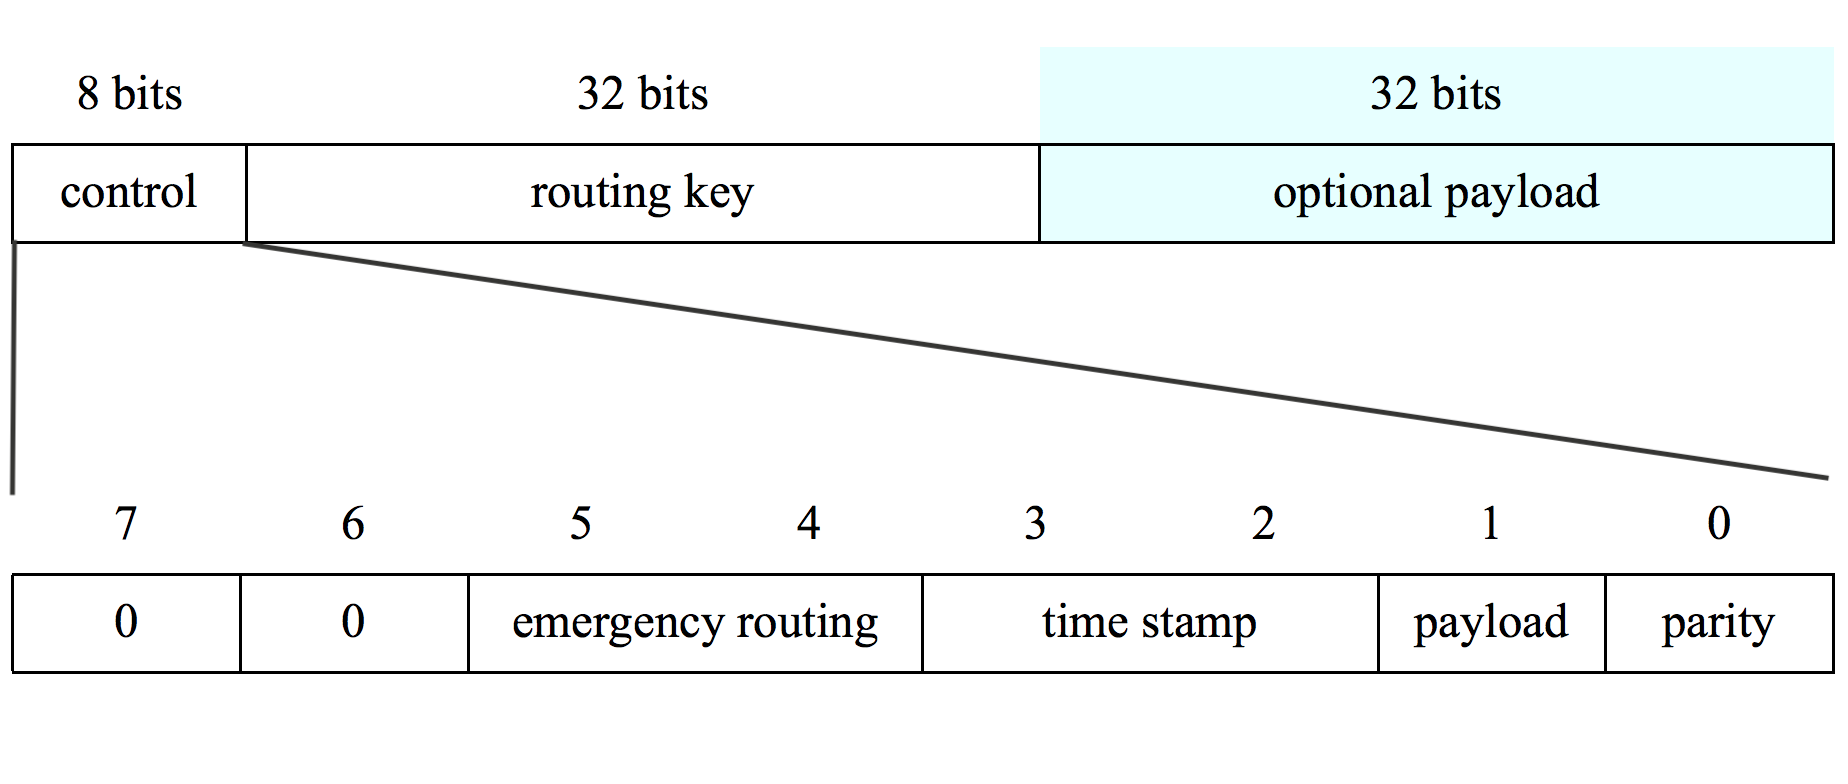
\includegraphics[width = 0.95\hsize]{figures/mc_pkt_layout.png}
\caption{Structure of a Multicast packet in SpiNNaker (image adapted from \cite{mc_pkt_layout}).}
\label{fig:mc_pkt_layout}
\end{figure}

As mentioned earlier, it is a 72-bit data frame where the routing key and the payload take up 32 bits each. Additionally, there are eight more bits of metadata that are used for management. The first two bits define the type of packet sent: \texttt{00} for MC, \texttt{01} for P2P, \texttt{10} for NN, \texttt{11} for FR. Then, the next two bits for emergency routing are stateful and can change depending on routing conditions. If a link fails or becomes congested at run time, this additional information will be updated and will help the local router find alternative routes. Then, the next two bits encode a global cycling four-step time stamp that is set by the packet sender. It allows late packets to be detected and dropped to ensure no \textit{errant packet} stays indefinitely in the network. Then, the payload bit signals if the packet has a payload or not. Finally, a parity bit is used to check for transmission errors. \\

Now that the physical components of SpiNNaker have been described, let us focus on the dense software stack that make this powerful tool usable.

\subsubsection{Software architecture} \label{sec:sw}

The software stack involved in a SpiNNaker simulation is summarised in Fig.~\ref{fig:software_stack}:

\begin{figure}[hbtp]
\centering
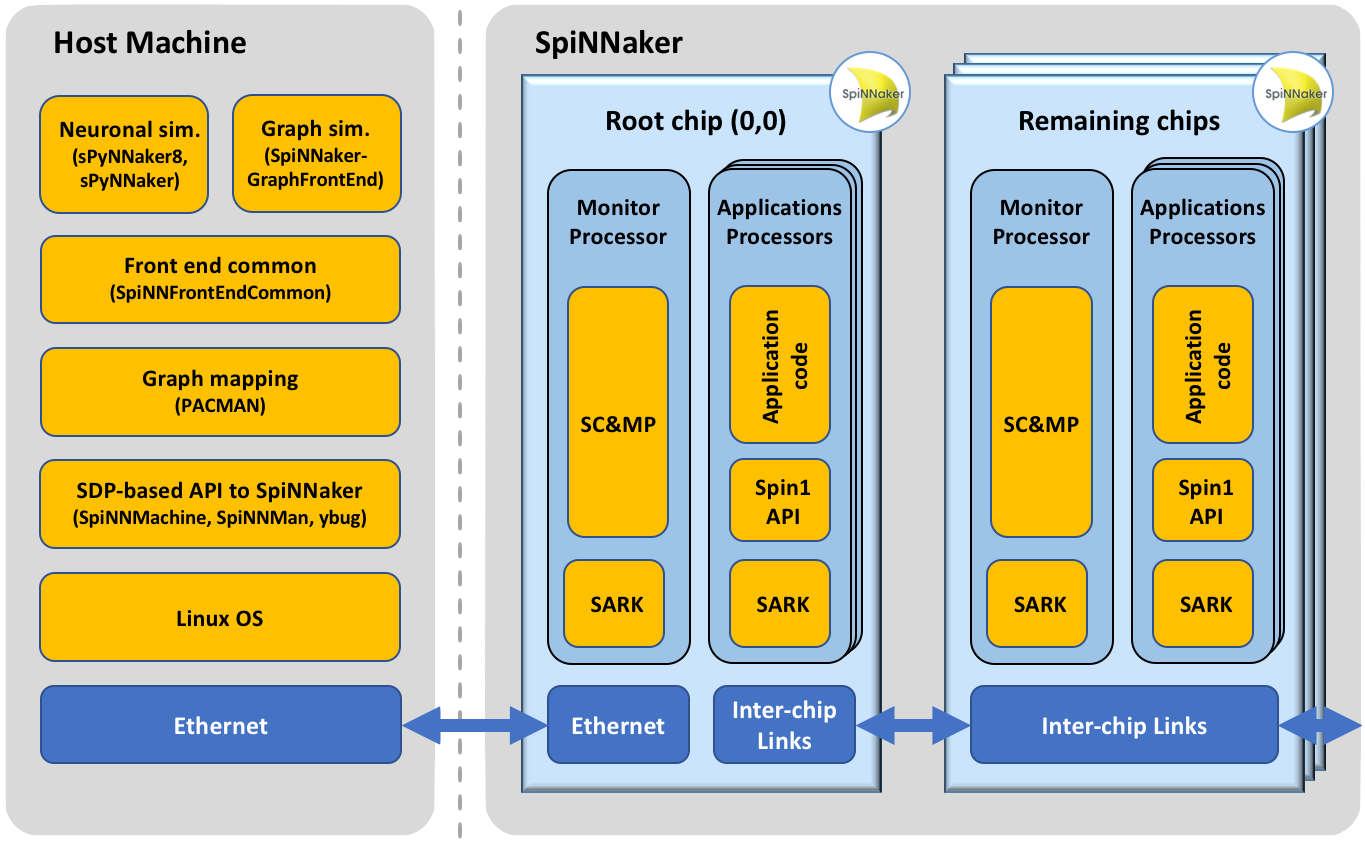
\includegraphics[width = 1\hsize]{figures/software_stack.png}
\caption{Structural diagram of the SpiNNaker software stack (image adapted from \cite{spinnaker}).}
\label{fig:software_stack}
\end{figure}

We will now detail thoroughly each module and its role within the entire stack. All these modules can be classified in one of the following three categories:

\begin{itemize}
\item \textbf{Host Machine}: this is the machine that the user is logged on, and where all the higher-level software resides. For example at the highest level, a spiking neural network simulation would be described in \texttt{sPyNNaker}, at a lower level neurons would be mapped to a SpiNNaker core in \texttt{PACMAN}, and even lower the compiled C application binaries sent to SpiNNaker through \texttt{SpiNNMachine}.

\item \textbf{Monitoring Processor}: runs the SpiNNaker Control and Monitor Program (SC\&MP) \cite{spinnaker} that contains all the monitoring-specific logic. At the foundation of any SpiNNaker core we also find the SpiNNaker Application Runtime Kernel (SARK) \cite{sark}. It is the lowest layer of software that provides functionalities such as core and application bootstrapping, memory management, interrupt control, handling of host machine commands on the monitor processor (e.g. remote memory alteration for debugging, application load / unload).

\item \textbf{Application Processor}: runs the simulation binary compiled from C on the host machine by the user. Two libraries providing support to the application code can also be statically linked with the binary. The first one is SARK, which is compulsory as it supports the application cores in the SpiNNaker environment. The second one is spin1, an event-based API that operates at a higher level and lets the user define callbacks for specific events.
\end{itemize}

All of these software tools will be detailed in turn in the following sections. The software running on the host machine is written in Python and binaries ran on SpiNNaker are first compiled from C on that machine as well. Then, the binaries are sent to the board for execution. \textit{Note}: in the following sections, we use the formatting convention \texttt{$\ll$Repository$\gg$} to name a software module that can be found on GitHub at \href{https://github.com/SpiNNakerManchester}{https://github.com/SpiNNakerManchester/$\ll$Repository$\gg$}.

\paragraph{Host Machine software}

The software stack running on the host machine is by far the most complex, because many distinct modules execute a specific task which is not always easy to grasp for the newcomer. Moreover, the user is likely to only directly touch the top layer of the stack which hardens a global comprehension of these modules. We will follow a top down approach to cover them all. \\

At the very top of the stack, there are two frameworks that can be used to define a simulation: \texttt{sPyNNaker8} for spiking neural networks and \texttt{SpiNNakerGraphFrontEnd} for generic graphs. The former, \texttt{sPyNNaker8}, is an implementation of PyNN, a \textit{simulator-independent language for building neuronal network models} \cite{pynn}. The software stack is actually further divided into \texttt{sPyNNaker}, a version-independent port of PyNN on SpiNNaker, and \texttt{sPyNNaker8}, a version-specific interface to sPyNNaker implementing PyNN version 0.8. This framework is specific enough that it can derive all the C application code from the high-level description of the simulation in Python. On the other hand, \texttt{SpiNNakerGraphFrontEnd} is a more generic framework and requires the user to define both Python graph specification and application code to be run on SpiNNaker. It makes it more flexible, but also makes the start-up cost of any serious project much higher as much of the logic needs to be handcrafted (e.g. routing). \\

A level below, there is \texttt{SpiNNFrontEndCommon} which holds all the common tools that are used by both front-end frameworks. For instance, it defines many 
Python abstract classes that define very specialised behaviours and that are combined together in the frameworks to create custom SpiNNaker elements. For instance, a Python class for a vertex in the \texttt{SpiNNakerGraphFrontEnd} could derive from the abstract class \href{https://github.com/SpiNNakerManchester/SpiNNFrontEndCommon/blob/master/spinn_front_end_common/abstract_models/abstract_has_associated_binary.py}{\textit{AbstractHasAssociatedBinary}} to indicate the class has an associated C code binary file. \\ % TODO: take a real example from a framework

Another level lower, this is the graph mapping algorithm called \texttt{PACMAN}. It takes as input the graph representing the simulation, whether it is a list of custom vertices or of interconnected neurons, and maps them to virtual SpiNNaker cores while complying with a given list of constraints. For instance, let us take the example of a graph of custom vertices that take up a lot of TCM such that a small number of vertices could fit on a SpiNNaker core without exhausting its resources. We would be able to call \texttt{PACMAN} with this graph and a list of constraints detailing the resource requirements of a single vertex, and \texttt{PACMAN} would figure out, say, only 100 of these vertices could fit on a single core and would return a mapping from the input graph to the virtual cores of the SpiNNaker machine. \\ 

Going another layer below, there is the ultimate collection of software modules that directly interact with SpiNNaker using SDP over UDP/IP. For a simulation triggered from one of the front-end frameworks, \texttt{SpiNNMan} will be used alongside one of its dependencies: \texttt{SpiNNMachine}. \texttt{SpiNNMan} is an interface to the SpiNNaker boards that is used by the higher layers to communicate with the machine. Consequently, it contains a set of functions that can be used to send messages to the board, spin up application cores, load binaries, and more. \texttt{SpiNNMachine} however is simpler and only provides a hierarchy of Python classes to represent the SpiNNaker machine. Finally, an interesting Command Line Interface (CLI) is \textit{ybug}, which can be found in the tool-kit repository \texttt{spinnaker\_tools}, and allows the user to directly interact with the machine. It is a Perl script that provides functionalities similar to \texttt{SpiNNMan} (e.g. cores boot, application loading, retrieving logs), but it runs as an interactive shell which empowers the developer with a practical solution for live inspection of the system. \\

As mentioned above, the SpiNNaker tools in \texttt{spinnaker\_tools} form another important module. It features the source code of important SpiNNaker binaries, such as SC\&MP, SARK and spin1, but also contains Perl scripts for tooling, such as ybug and some more visualisation GUIs not used by that project. \\

All in all, the software stack of the host machine piles up relatively high, and a good overview of the role of each module is a significant edge towards becoming a proficient SpiNNaker developer. Now let us focus on the binaries that run on SpiNNaker (after being compiled and transferred from the host machine).


\paragraph{Monitoring Processor software}

\begin{figure}[hbtp]
\centering
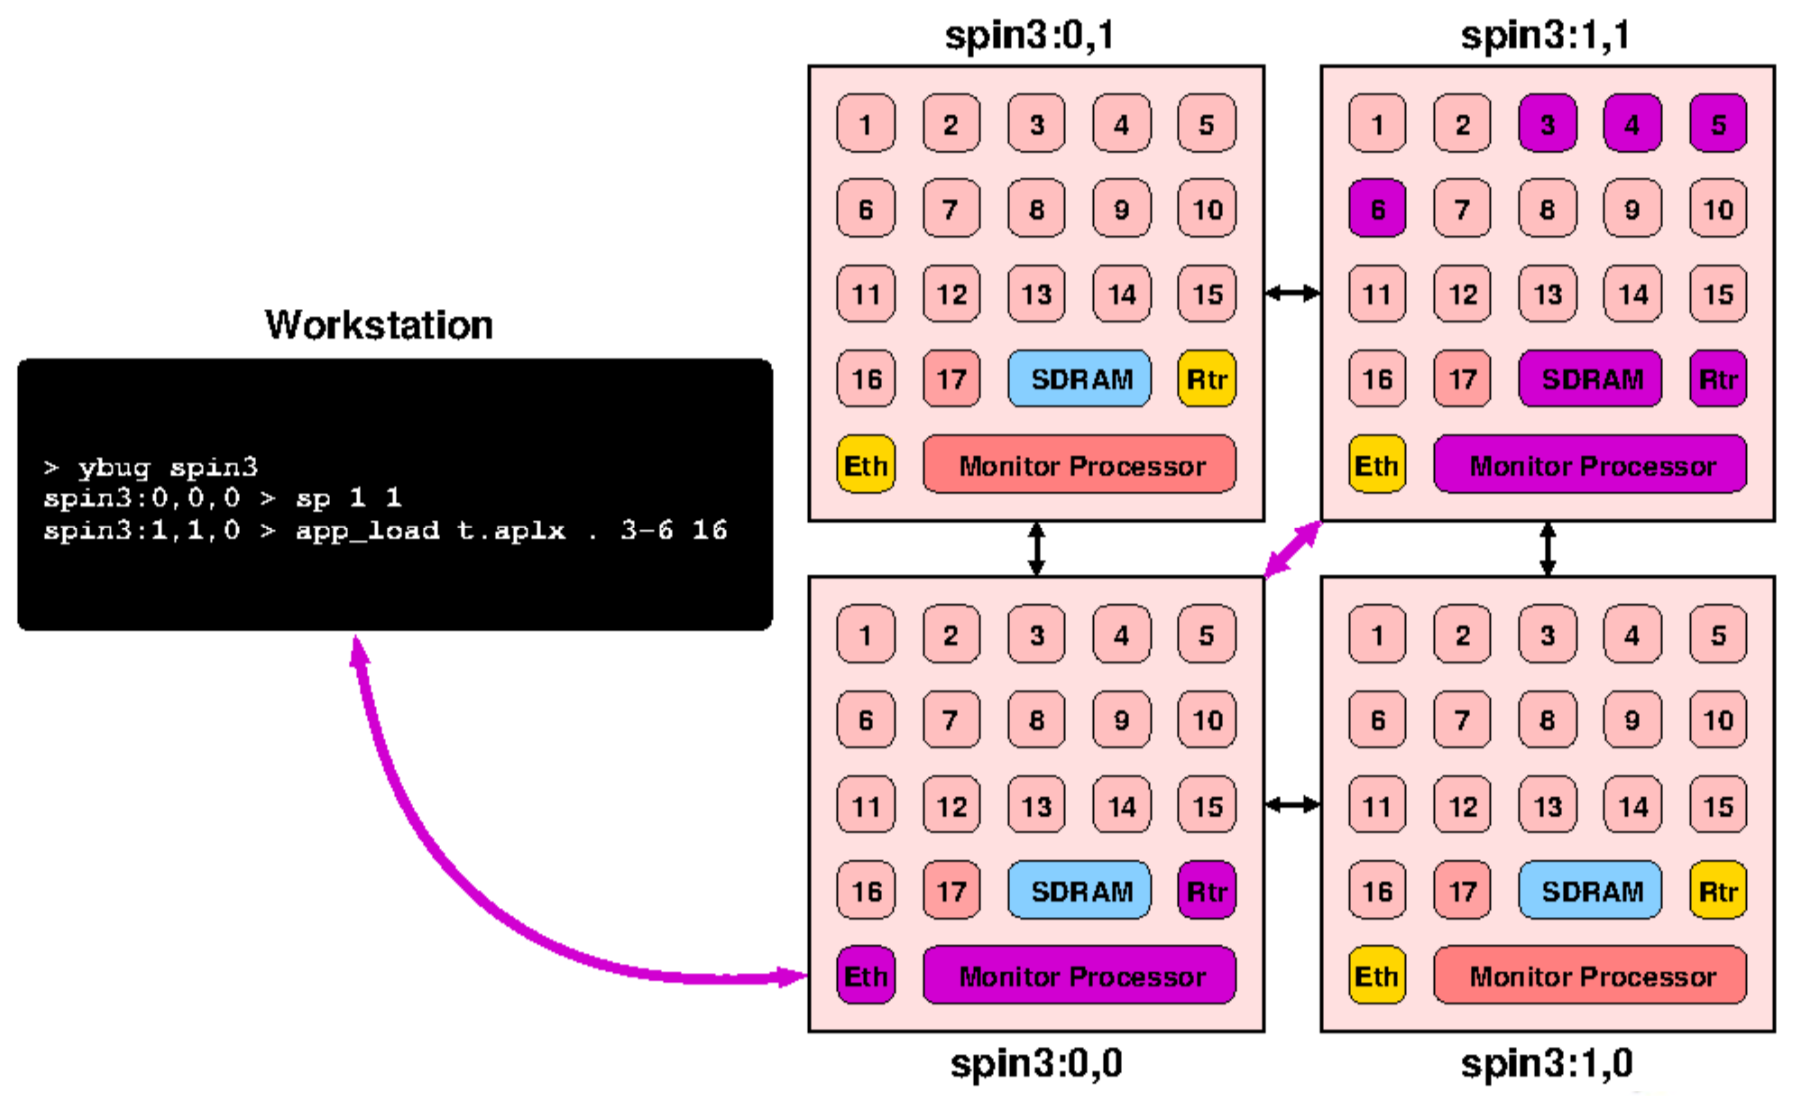
\includegraphics[width = 1\hsize]{figures/ybug.png}
\caption{Application loading using \textit{ybug} (image from \cite{ybug}).}
\label{fig:ybug}
\end{figure}

Focusing now on the Monitoring Processor, the main software component is the SpiNNaker Control and Monitor Program (SC\&MP). The program is loaded on all the monitoring cores during the system bootstrapping phase and oversees the operations of an entire chip. It handles any command received from the host machine using the SpiNNaker Command Protocol (SCP) \cite{ws6} (transmitted over SDP), and executes them. For the monitoring processor on the \textit{root} chip (on board directly connected to the host machine), SC\&MP will also inject in the SpiNNaker network any inbound packet received from the host. For instance, if a developer uses \textit{ybug} to load application \textit{t.aplx} on cores 3 to 6 of chip (1,1) with the application ID 16, the generated SDP packets would cross the hardware elements shown in Fig.~\ref{fig:ybug}. \\

Another important piece of software is the SpiNNaker Application Runtime Kernel (SARK) \cite{sark} library. It is required on all SpiNNaker cores and implements the following three functionalities:

\begin{itemize}
\item \textbf{Bootstrapping}: initialises all cores, memory stacks and control registers. Then, it calls the application \textit{c\_main} function which acts as the \textit{main} of a C program: it is the entry point of the application code that starts the simulation.

\item \textbf{Utility tooling}: for low-level interaction with the chip, e.g. memory management, interrupt controller, LEDs state update. It also implements some higher-level constructs, such as per-core 8-bit semaphores that are implemented using a combination of DTCM and hardware locks.

\item \textbf{Extra tooling for monitoring processor}: mainly to handle host machine commands using SCP/SDP (SpiNNaker Command Protocol over the SpiNNaker Datagram Protocol). This is the code that will handle any ybug-issued command targeted at the chip it is on.
\end{itemize}

Finally, let us see the application cores which run the code written by the developer.

\paragraph{Application Processor software}

On all application cores, SARK will need to be loaded as well as it provides the basic and compulsory framework for any application binary. Additionally, an optional library can be linked with the application binary and provides support for an event-based API. In SpiNNaker's manycore paradigm using message passing, it is likely the developer will want most (if not all) of the logic of its simulation to run as an event handler. For example in a spiking neural network, the application code will want to handle incoming spikes arriving and potentially propagate a new spike as a response to that event. To help the developer in doing so, the SpiNNaker Application Programming Interface (API), abbreviated \textit{spin1}, was built. It allows the user not to worry about the control flow of its simulation and only focus on the data flow by defining callbacks. Four types of events can be handled \cite{spinnaker}: 

\begin{itemize}
\item \textbf{Incoming packet}: handle a packet that just arrived. A different callback can be registered for each of the four types of packet that can be received (see section \ref{sec:pf}).

\item \textbf{DMA complete}: when the DMA controller finished an operation.

\item \textbf{Timer tick}: to implement time awareness, the core 'ticks' every millisecond (configurable) to increment its local notion of time.

\item \textbf{User event triggered}: it is a software-triggered interrupt to let the user handle a custom event.
\end{itemize}

Each of these callbacks can be dynamically registered and unregistered at runtime using \textit{spin1}. Moreover, a priority needs to be given to each of these callbacks at registration to define which callback should run first when two events occur at the same time. As in Unix niceness for processes, the lower the value of that priority, the higher the priority. Two different types of priorities can be registered:

\begin{itemize}
\item \textbf{Queueable callbacks}: their priority value is $\ge 0$. If a callback with a lower priority value is already running, they will be queued by the scheduler. However, they will pre-empt any running callback with a higher priority value.

\item \textbf{Non-queueable callbacks}: their priority is $-1$. They execute immediately without possibility of being interrupted, pre-empting any running callback. For this properties to hold at any time, only a single non-queueable can be defined per core. Otherwise, if two such callbacks were defined and triggered at the same time, one would end up pre-empting the other or one would not be executed immediately.
\end{itemize}

Overall, these libraries equip the developer with a comprehensive set of tools that let simulations be defined at different granularities. Now that we have described the set of tools available to us, developers who want to port Page Rank to SpiNNaker, let us review how SpiNNaker can actually be used. \\

\subsection{SpiNNaker usage} \label{sec:usage}

As explained, SpiNNaker (Spiking Neural Network Architecture) was built for spiking neural networks simulations. This is the reason why a lot of effort was put into having the \texttt{sPyNNaker} / \texttt{sPyNNaker8} front-end frameworks expose a very high-level API entirely in Python. It makes the tool very user-friendly and enables researchers to quickly craft a simulation without bothering with its implementation technicalities. We will first be discussing spiking neural network simulations in section \ref{sec:snn}, and will then focus on alternatives applications of SpiNNaker together with their implementation in section \ref{sec:aa}. All the use cases described will be relevant because the design decisions of the Page Rank implementation in this project depends on an understanding of the benefits and drawbacks of each example's approach.

\newpage % TODO: remove me
\subsubsection{Spiking neural networks} \label{sec:snn}

First, let us go through a brief biology refresher to properly define what a neuron, an axon and a synapse are.

\begin{figure}[hbtp]
\centering
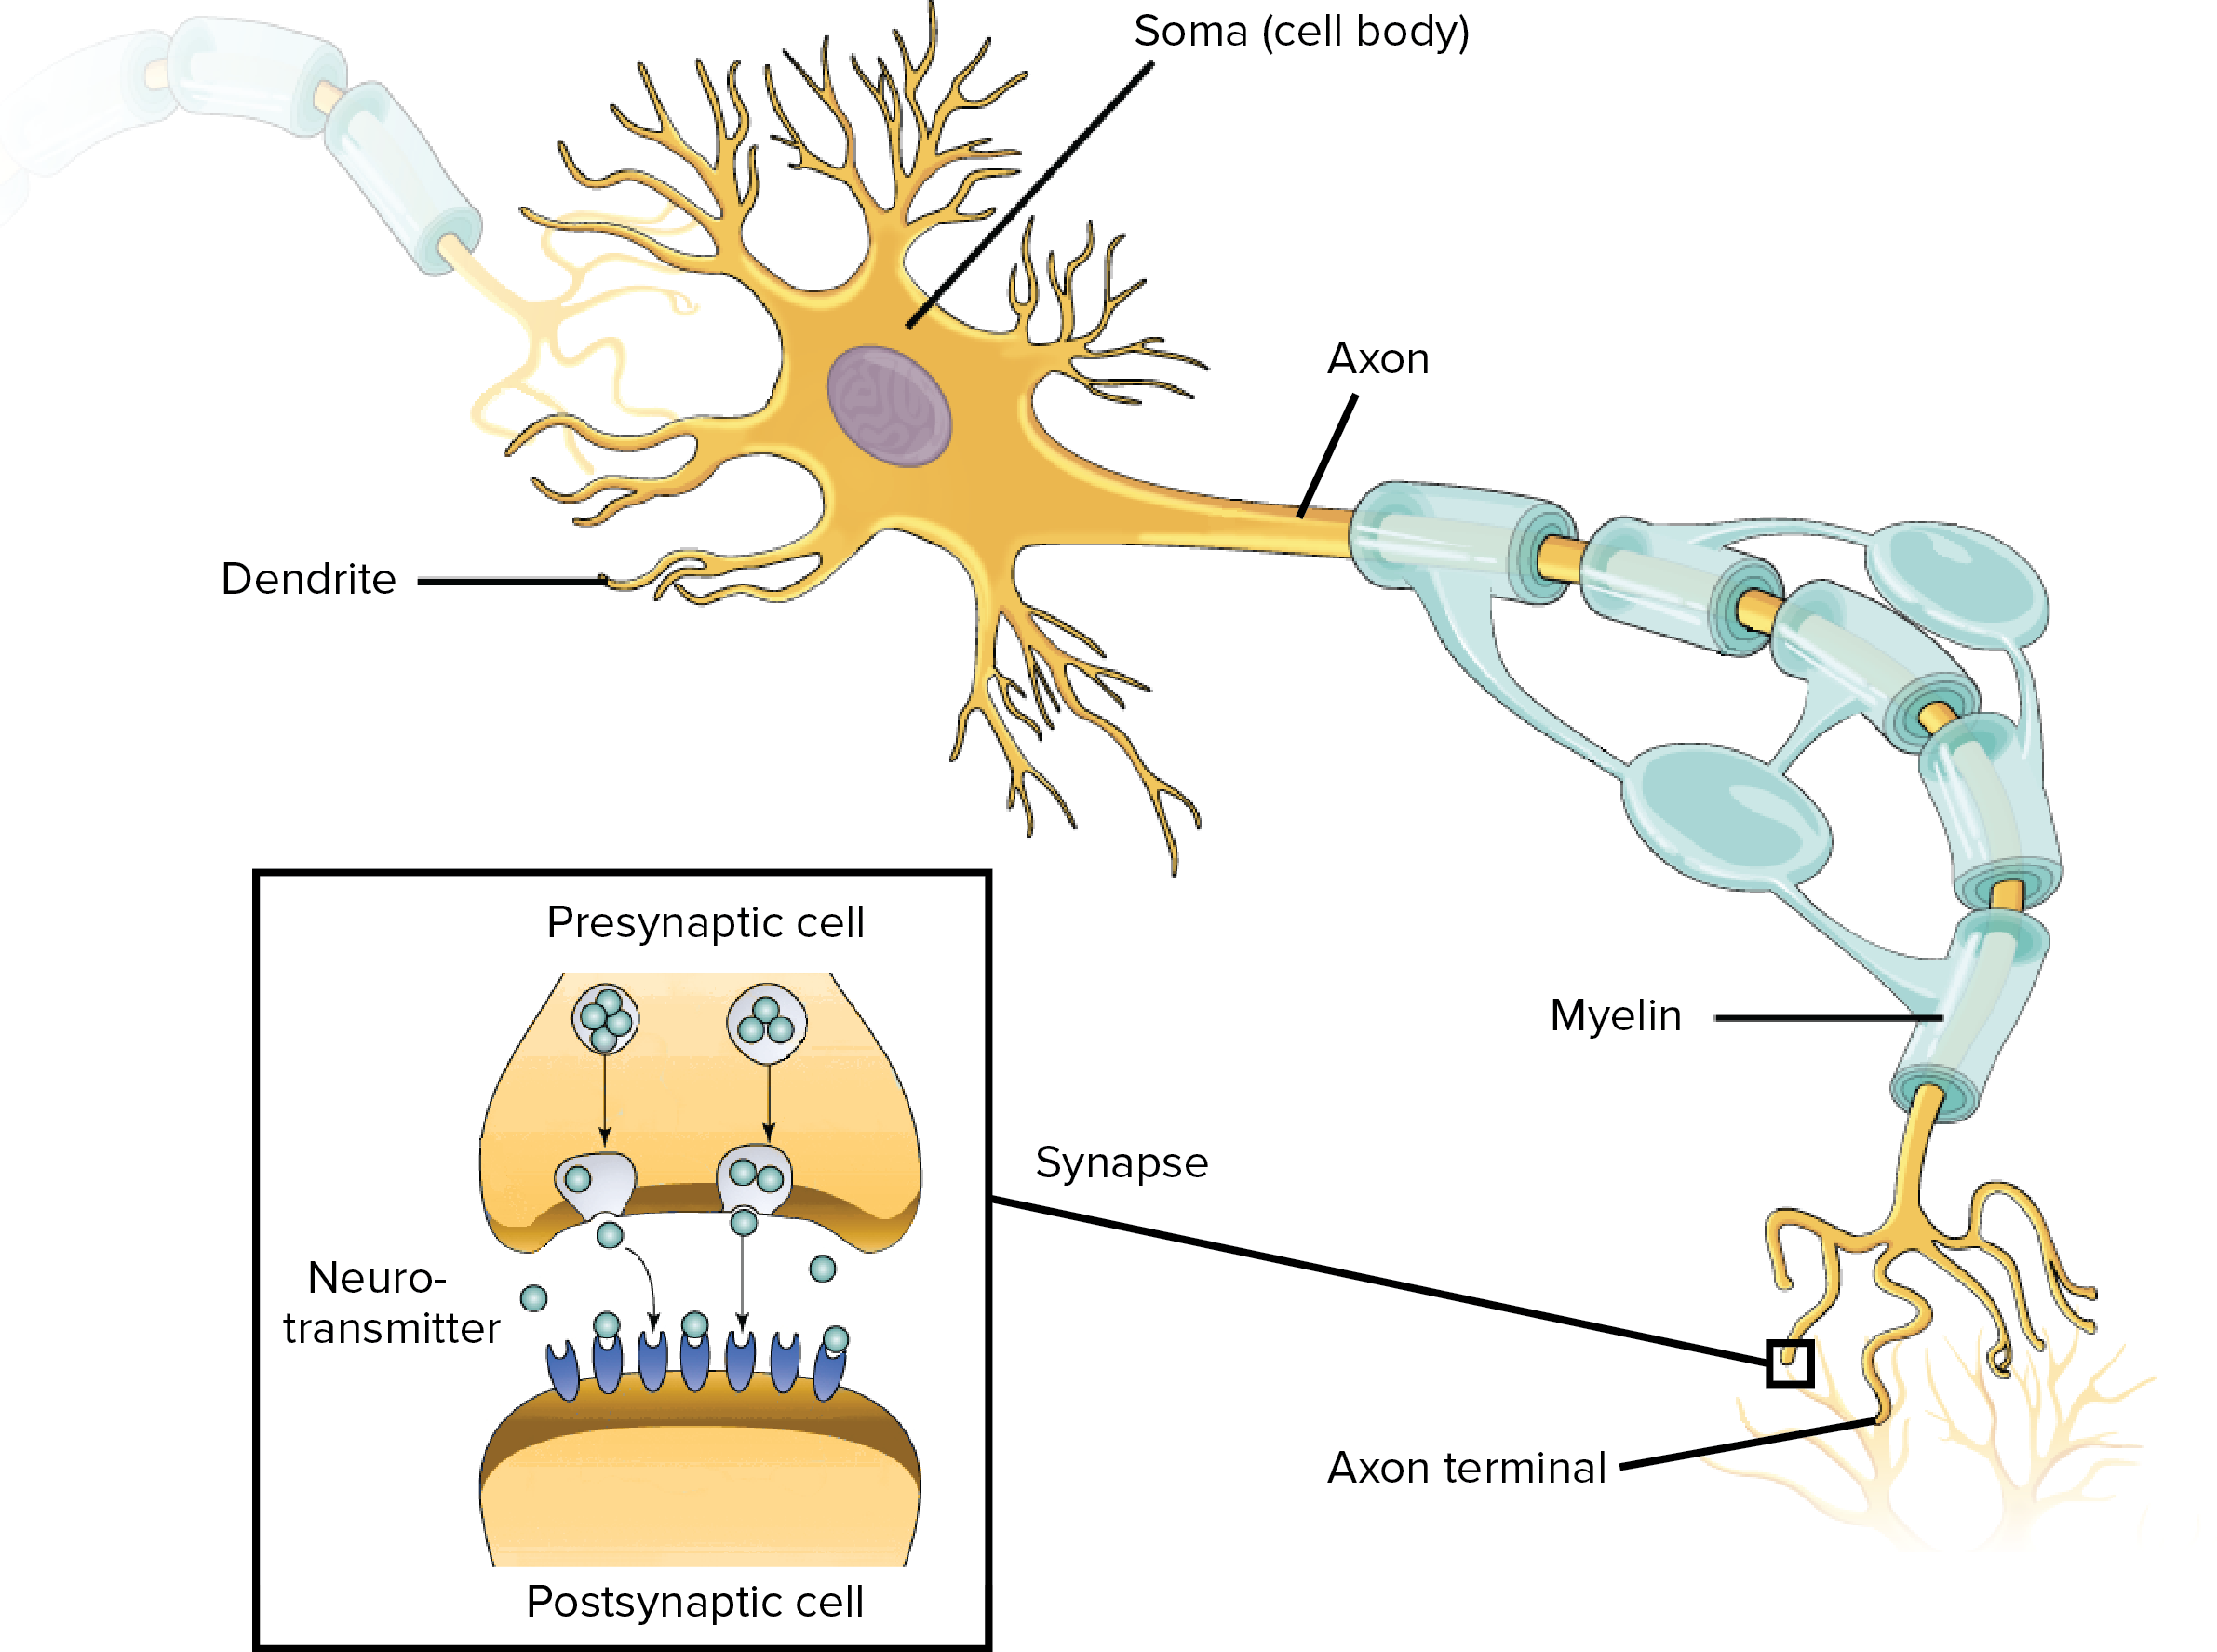
\includegraphics[width = 1\hsize]{figures/neuron.png}
\caption{Structure of a neuron with one of its synapse (image adapted from \cite{neuron}).}
\label{fig:neuron}
\end{figure}

On Fig.~\ref{fig:neuron}, there is a neuron with the \textit{Soma} being its body. \textit{Neurons} are the building blocks of the human brain and their electrical current generates \textit{action potentials}, also called voltage \textit{spikes}, when reaching an excitatory state. Each \textit{neuron}'s voltage is modulated by incoming spikes received from its \textit{dendrites}, and can send out spikes of its own through \textit{axon terminals}. All spike exchanges occur in the \textit{synapse}, where \textit{neurotransmitters} from the \textit{pre-synaptic cell} (axon terminal) will be transferred to the \textit{post-synaptic cell} (dendrite), which will update the voltage in the neuron. When this voltage hits a certain threshold, the neuron \textit{fires} a voltage \textit{spike}. Then, the \textit{spike} goes through the \textit{axon}, accelerated by the \textit{myelin} structure, and frees neurotransmitters in the outbound synapses which will in turn propagate the spike to other neurons. \\

Two main classes of models are implemented in \texttt{sPyNNaker}, describing how neurons fire in response to incoming spikes (neuron models) or describing how synapses transfer spikes based on parameters such as spike \textit{frequency} or \textit{time interval} (synapse model). The details of these models are not relevant for the needs of this Page Rank project, but we still show below a minimal example of a spiking neural network simulation. The example below (adapted from \cite{pynnsim}) uses the \texttt{IF\_curr\_exp} neuron model and the \texttt{StaticSynapse} synapse model, which are defined in PyNN \cite{pynn} but not detailed here as they are not relevant for the project. \\

\begin{minted}{python}
import spynnaker8 as sim

# Setup SpiNNaker with for 1 microsec time steps
sim.setup(timestep=1.0)

# Define a population of 1 neuron that will spike once at time t=0
pIn = sim.Population(1, sim.SpikeSourceArray(spike_times=[0]), label="input")
# Define a population of 1 neuron with neuron model `IF_curr_exp'
pOut = sim.Population(1, sim.IF_curr_exp(), label="output")
# Define a synapse link pIn -> pOut with synapse model `StaticSynapse'
sim.Projection(pIn, pOut, sim.OneToOneConnector(),
               synapse_type=sim.StaticSynapse(weight=5, delay=1))

# Set spikes and voltage to be recorded at each time step
pOut.record(["spikes", "v"])

# Starts the simulation
sim.run(10) # simulation run time in ms

# [Omitted] Collect and display recorded data...
\end{minted}

This example creates a neural graph where two populations (i.e. groups) of one neuron each are linked together by a directed arc from \texttt{pIn} to \texttt{pOut}. Using biology terms, this means we define the neuron in \texttt{pIn} to have an axon linked to a synapse with a dendrite of the neuron in \texttt{pOut}. Then, we indicate we want the simulation to record the voltage over time of the receiving neuron together with to time steps when a spike was fired. Finally, we can run the simulation for 10 milliseconds and display the recorded data as shown in Fig.~\ref{fig:simple_spynnaker8}. The full code is given in Appendix \ref{app:a}.

\vspace{-0.1cm}
\begin{figure}[hbtp]
\centering
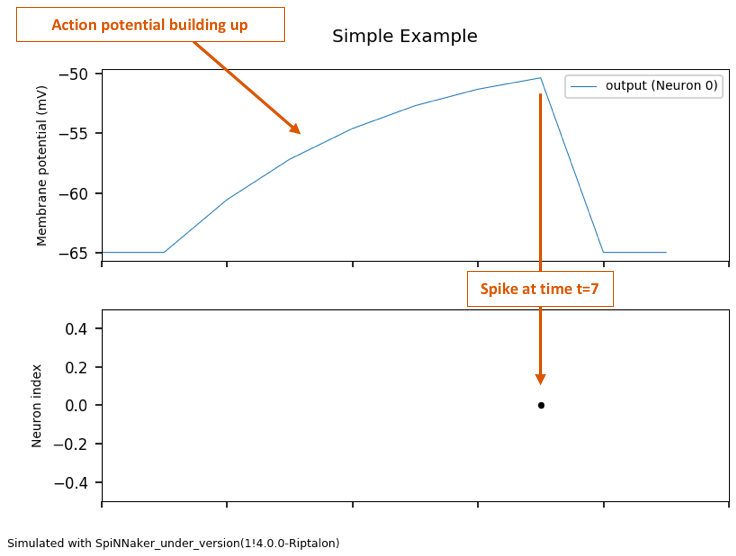
\includegraphics[width = 0.8\hsize]{figures/simple_spynnaker8.png}
\caption{Voltage and spikes fired over time \texttt{sPyNNaker8} simulation.}
\label{fig:simple_spynnaker8}
\end{figure}

This example is quite intuitive and straightforward, so we can image that even for complex simulations the implementation on sPyNNaker will not be a challenge. However, this framework is very specific and, for reasons detailed in the project section \ref{sec:impl}, Page Rank computations cannot be expressed in this framework. Consequently, we also give some background for alternative applications of SpiNNaker, those that cannot be expressed as spiking neural networks and that are still efficiently computed on SpiNNaker. \\

\subsubsection{Alternative applications} \label{sec:aa}

When the targeted application is not a spiking neural network, \textit{sPyNNaker8} is usually too constraining as it is high-level and makes design assumptions that only fit a spiking neural network.

\paragraph{Heat Equation Solver} \label{sec:hes}

To illustrate this issue, let us take the example of a heat equation solver running on SpiNNaker. Such a simulation is defined by a 2D grid where each cell iteratively propagates its heat to its neighbours according to a fixed set of rules. The algorithm propagates heat step-by-step until a convergence point is reached at time $k$, that is when the L1-norm $|| \textnormal{grid}_k - \textnormal{grid}_{k-1} ||_1 $ is less than a given threshold. Regarding the SpiNNaker implementation, a design requirement that disqualifies \texttt{sPyNNaker8} upfront is the need for each node to propagate some of its state (its heat). Indeed in the \texttt{sPyNNaker} implementation, each neuron is managed alongside its inbound synapses. When a neuron A spikes and it points to neuron B, A will send a packet to tell neuron B it spiked but without carrying any information about the intensity of the spike (40-bit packet with no payload, see \ref{sec:pf}). This is because all spikes have the same intensity (configurable in simulation parameters) and modelling a smaller spike is delegated to the synapse. Consequently, no state can leave the neuron which conflicts with the requirement for a heat node to propagate some of its local heat. \\

\begin{wrapfigure}[18]{r}{0.5\textwidth}
    \begin{center}
    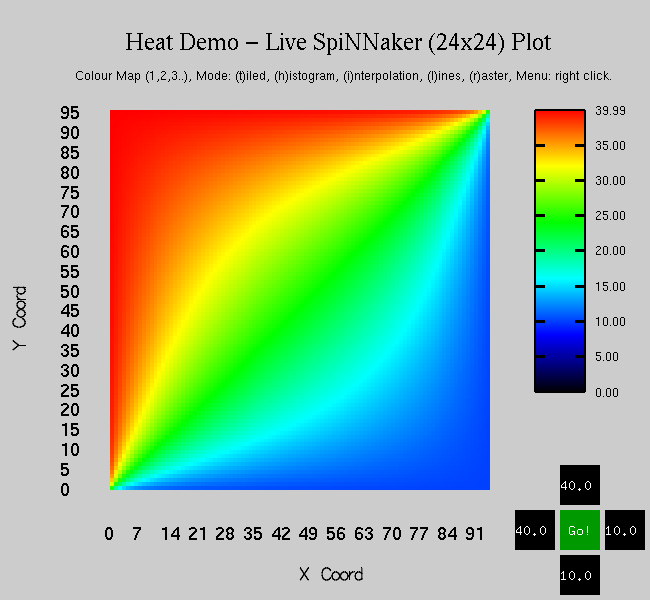
\includegraphics[width=0.48\textwidth]{figures/heatvis.png}
  	\caption{The visualiser for the Heat Equation solver (image from \cite{heatvis}).}
  	\label{fig:heatvis}    
    \end{center}
\end{wrapfigure}

As a result, the \texttt{SpiNNakerGraphFrontEnd} was chosen to implement the heat equation solver, which can be found in an earlier version of the examples shipped with the module \cite{gfeheat}. The solver also had a visualiser that was directly exchanging SCP/SDP packets with SpiNNaker to show a live view of the grid with its heat converging; see Fig.~\ref{fig:heatvis}. Part of the tooling kit built for SpiNNaker involves a few visualising tools which we do not use for this project. This particular visualiser is a custom one made solely for the purpose of this example, but it relies of the same patterns as the general-purpose ones. \\


\paragraph{Markov Chain Monte Carlo Inference (MCMC)} \label{sec:mcmc}

This last example is also very relevant for us as implementing MCMC requires the propagation of some state across the system. Like the Heat Equation Solver, the data flow moves across the network. The results of this project were published in a paper \cite{markov-on-spinn} co-authored by Steve Furber, the head of the Advanced Processor Technologies Group (APT) at the University of Manchester that designed SpiNNaker. \\

The project uses Neural Sampling and Gibbs sampling with Bayesian networks as a benchmark to test the computational abilities of SpiNNaker machines on alternative applications. Running these models is very CPU-intensive and offers parallelism opportunities, hence the choice of SpiNNaker. Implementation-wise, the \texttt{SpiNNakerGraphFrontEnd} was also used and a framework was built around it to let researchers define new Markov Chain models. \\

In addition to the design decisions made, the interesting takeaway from that project is the scaling results observed, see Fig.~\ref{fig:markov-spinn-results}:

\begin{figure}[hbtp]
\centering
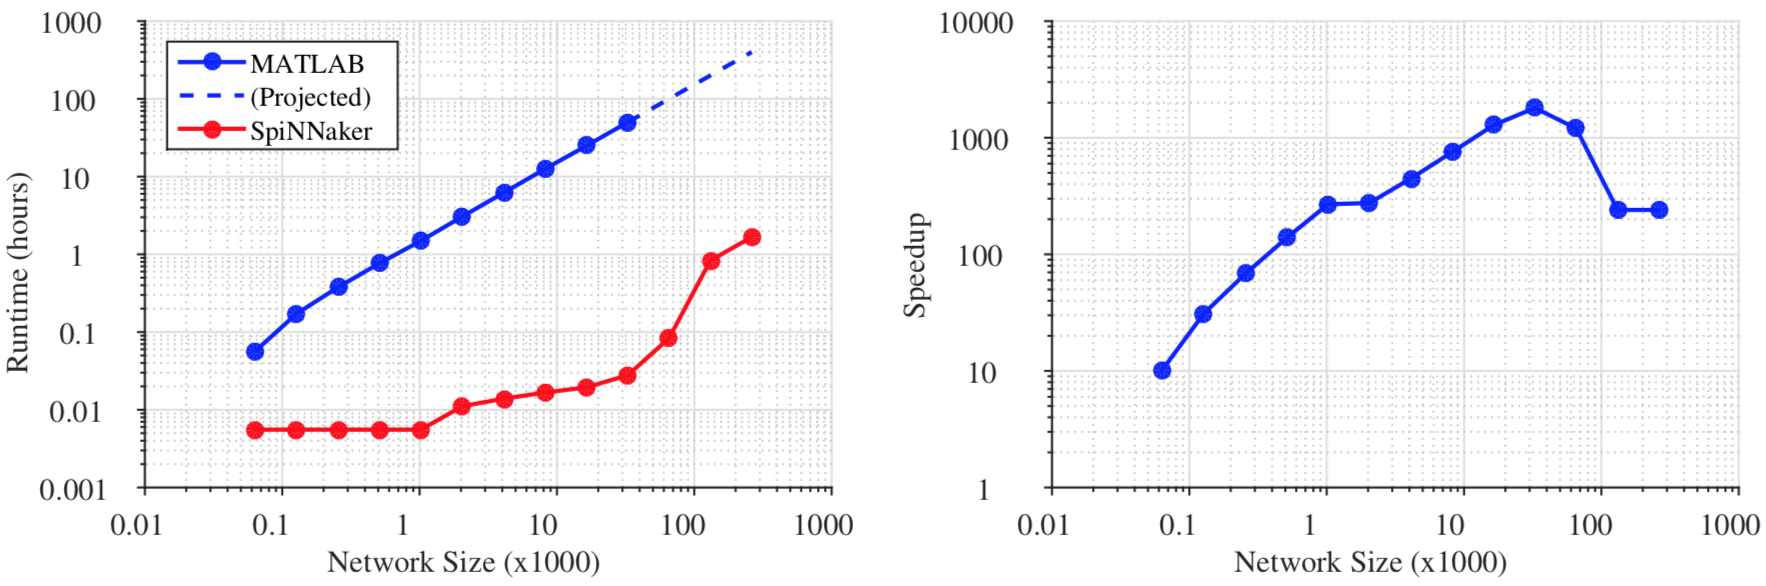
\includegraphics[width = 1\hsize]{figures/markov-spinn-results.png}
\caption{Runtime and speedup comparisons between 50,000 iterations of single-threaded Neural Sampling on a PC (Intel Core i7 3770K processor) in MATLAB and parallel Neural Sampling with spiking neurons on SpiNNaker (48 chips) (image and caption adapted from \cite{markov-on-spinn}).}
\label{fig:markov-spinn-results}
\end{figure}


First of all, we can note that it is probably inconsistent to compare the running times of two machines of such a different nature, so we will not be concluding anything from the running times alone. \\

Nonetheless, the scaling curves on each machine (a unit-less version of the runtime graph on Fig.~\ref{fig:markov-spinn-results}) are very relevant. We can observe that the simulation scales linearly on a PC whereas on SpiNNaker the scaling is sub-linear up to a network size of 100,000 nodes. [TODO: try to relate to the resources used to explain it if possible...] This trend motivated projects like this one, by demonstrating that the scaling potential on SpiNNaker was significant. It also exhibits another potential pitfall of SpiNNaker, which relies on a network to propagate messages. The drop in performance from 100,000-node graphs is due to network congestion that physically limits the scalability potential of algorithms that need to exchange too much state at once. This will be a parameter to look for in this project's implementation of Page Rank: can we anticipate a drop in performance for some given graph topologies? \\

\vspace*{-0.1cm}
Having covered all the background material needed, we can now review the successive implementations that constitute one of the contributions of this project.


\newpage
\section{Page Rank on SpiNNaker} \label{sec:impl}

This section will be discussing the main contribution of this project: a Page Rank simulation framework on SpiNNaker which we discuss in section \ref{sec:prsf}. Beforehand, we also review in section \ref{sec:tool} an important preparatory phase which is related to tooling. \\

All the source code is available at: \url{https://github.com/louisblin/FYP}.

\subsection{Tooling} \label{sec:tool}

\subsubsection{Dependencies and environment management}

Developing for SpiNNaker is a dependency-hungry activity. Indeed, the project requires both hardware and complex software dependencies that are not clearly stated in a unique documentation guide. \\

The first dependency lies in the hardware. We were fortunate enough to have access to a SpiNNaker 4-chip board (Spin3 - see Fig.~\ref{fig:spin3}) for the needs of this project. Then, only an Ethernet cross-over cable is needed to directly connect the network interfaces of SpiNNaker and the host machine, and the set up remaining is done at the software level. \\

The biggest start up cost is with the software. This project was challenging in many aspects, and a significant part of it was due to the steep learning curve required to understand the SpiNNaker paradigm. First, the difficulty   arises from the complex dependency tree that needs to be understood by the newcomer. We will see that there are no less than 14 software modules (\texttt{sPyNNaker}, \texttt{sPyNNake8}, etc.) that the Page Rank framework, or any SpiNNaker simulation as a matter fact, needs to import. Additionally, there are restrictive constraints on the Operating System (OS) that can be used to compile and run these modules. Although the SpiNNaker team advertises the software stack is cross-platform, which it probably is, the outdated installation guides do not allow the unaided newcomer to easily install these dependencies on any machine. In practice, the easiest way to get started is to use Ubuntu 14.04 on a Virtual Machine (VM), and then run the provided examples to confirm the installation was successful. Here again, the user has to guess the authors probably used that Linux distribution to develop their software, but this is not clearly stated in the documentation. Finally, the exact same build tools, such as \texttt{gcc} together with a specified version, have to be used to compile all the C source files properly. Below is an annotated directory listing of the project dependencies (those ending with a '\textit{*}' were not mentioned in the background section for the sake of simplicity, as they are not relevant this project):

\begin{verbatim}
$ tree -L 1 .
.
|- DataSpecification*      # Formats host machine <-> SpiNNaker data 
                             exchanges
|- gcc-arm-none-eabi*      # The gcc build suite
|- PACMAN
|- spalloc*                # SpiNNaker machine allocation client, for 
                             shared machines
|- SpiNNakerGraphFrontEnd
|- spinnaker_tools
|- spinn_common*           # Mixed C utilities
|- SpiNNFrontEndCommon
|- SpiNNMachine
|- SpiNNMan
|- SpiNNStorageHandlers*   # Host-based Storage I/O handler classes
|- SpiNNUtils*             # Mixed Python utilities
|- sPyNNaker
|- sPyNNaker8
\end{verbatim}

All in all, this start-up cost could be easily manageable provided the documentation was written for unaided newcomers. Indeed, much of the documentation makes the assumption new users will be introduced to SpiNNaker via one of the yearly workshops and that the very basics will be explained orally. A good example for that would be the versioning system, where the documentation does not explain that all software modules define \texttt{git tags} versions that should be matched across modules. Also, git tags on GitHub are not sorted chronologically, and the documentation does not explain version \textit{2016.001} is supposed to come before version \textit{4.0.0}. At least the former issue is invisible when installing dependencies through \texttt{pip}, which is configured to find the right versions, but it needs to be autonomously understood when installing from source. \\

Installing from source was compulsory for the needs of this project as the source files from this project's implementation are jointly built with those of \texttt{sPyNNaker}. Moreover, it has the benefit of helping the newcomer understand the structure of the project. Indeed, it requires all nested dependencies to be installed by hand and it enables the newcomer to visualise rapidly which module relies on what other one. Another significant upside of this installation is that it keeps all the C source files that structure some of these modules. As an example, \texttt{sPyNNaker} builds a number of binaries that are installed in the Python source tree of the project and that can be loaded on SpiNNaker. Installing through \texttt{pip}, which contains the pre-compiled C binaries already installed, would have hidden that build process of the C code and hardened a global understanding of the software stack. \\

To cope with the issue of managing such a specific environment, it was decided to \textit{containerise} the project. This is detailed in the next section as it can be of interest for anyone working with SpiNNaker and needing a solution for environment management, independently of the scope of this project. \\

\begin{figure}[hbtp]
\centering 

\includegraphics[width=1\hsize]{figures/docker-banner.png}
\caption{The Docker logo (image from \cite{docker}).}
\label{fig:docker}
\end{figure}

\subsubsection{Docker}
% NOT AS A BLOG

Docker is a leading platform offering containerisation services \cite{docker}, which are essentially a lighter version of virtual machines. Choosing Docker comes with the following benefits:

\begin{itemize}
\item \textbf{Lightweight}: container provide properties comparable to virtual machines but at a lower resource footprint. This applies both to the start-up cost, which is under a second for a container, and to the CPU overhead during operations that is also negligible.

\item \textbf{Environment} management: containers are self-contained environments, in which all the \textit{pre-installed} software dependencies of the project can be embedded. Ironically, it is by introducing a new dependency on Docker that we solve this dependency management problem, by encapsulating all the build logic of each module into a Docker image. Additionally, new fresh environments can be created on demand at a low cost, which solves the environment management problem.

\item \textbf{Portability} of the deliverables was an important design decision from the start, as this project hopes to be a starting point for further investigation using SpiNNaker. A tool that can easily be run on any platform with a low start-up cost highly contributes to making it user-friendly. As an example, after having cloned the project and installed Docker, a one-liner command is enough to run an example from this project.
\end{itemize}

As a side note, the ability of Docker to hide all the cumbersome details of environment management while providing portable performance, is well illustrated by Docker's logo, see Fig.~\ref{fig:docker}. \\

Having selected Docker for containerisation, we build the following two images that each target a different application:

\begin{itemize}
\item \textbf{Developer tool-chain} (\href{https://hub.docker.com/r/louisleblin/toolchain/}{\texttt{louisleblin/toolchain}} on Docker): this is the most complex image, which contains all the necessary software modules compiled from source, as explained above. This tool-chain provides the right environment for SpiNNaker developers, as well as the build tools used to compile the entire SpiNNaker project. Two versions of the tool-chain are available via Docker tags: versions \textit{2016.001} and \textit{4.0.0} respectively via tags \texttt{v2016.001} and \texttt{v4.0.0}.

\item \textbf{User sPyNNaker8}  (\href{https://hub.docker.com/r/louisleblin/pynn8/}{\texttt{louisleblin/pynn8}} on Docker): this is intended for SpiNNaker users running spiking neural network simulations using \texttt{sPyNNaker8}. This image is available via the default Docker tag \texttt{latest} .
\end{itemize}

Placing user-friendliness as a central requirement of the project, these production images were not convenient to use as an interactive shell, which has been their most common use case over the course of this project. Consequently, each image is released under two versions: (a) a production version containing the minimal set of dependencies and (b) a development version, built from the production image, featuring additional development tools such as \textit{vim}, a custom \textit{zsh} shell, and more. The images mentioned are summarised in Table ~\ref{table:a} below: \\

\begin{table}
\begin{center}
\begin{tabular}{ |l|l|c| }
 \hline
\textbf{Image name} & \textbf{Image tag} & \textbf{Compressed size}  \\ 
 \hline
louisleblin/toolchain & v2016.001 & 438 MB \\ 
louisleblin/toolchain & v2016.001-dev & 636 MB \\ 
louisleblin/toolchain & v4.0.0 & 616 MB \\ 
louisleblin/toolchain & v4.0.0-dev & 459 MB \\ 
louisleblin/pynn8 & latest & 379 MB \\ 
louisleblin/pynn8 & dev & 415 MB \\ 
 \hline
\end{tabular}
\end{center}
\caption{Docker images available at \url{https://hub.docker.com/r/louisleblin}}
\label{table:a}
\end{table}

Finally, a work-flow that proved to be successful for this project was to use Travis CI to rebuild and publish these images on Docker Hub. On every push on the master branch, Travis spawns three processes that each rebuild a production / development pair of images from Table ~\ref{table:a}. First, the latest published image is pulled from Docker Hub and the \texttt{git commit} hash it was tagged with is extracted. Then, a \texttt{git diff} between that extracted commit and the current commit allows to check whether any relevant files have changed. If it is the case, a new image is built, tagged with the current commit hash and pushed to Docker Hub. Otherwise, the process terminates, having skipped the rebuild. \\

The main benefits of this approach are the consistent and reproducible image build and publication processes, that add to the convenience of automating these builds on a remote platform. See the project repository for further details, under \texttt{scripts/docker\_*} for triggering rebuilds / publications from Travis and under \texttt{docker/* } for the build logic of each image.  \\

Finally, it is noteworthy to mention that no such Docker images were found prior to that project, so this is already a tooling contribution that might be of help for SpiNNaker developers and users. Using these tools greatly helped with the development process of the Page Rank simulation framework, which we detail in the following section. \\

\subsection{Page Rank simulation framework} \label{sec:prsf}

This Page Rank simulation framework is the main contribution of this project. We will first review early attempts and resulting design considerations in section \ref{sec:des}. Then, we will have the means to focus on the final implementation in section \ref{sec:implementation}.

\subsubsection{Design considerations} \label{sec:des}

\paragraph{Approach 1 - sPyNNaker}

The simplest approach one can take to run Page Rank on SpiNNaker is to try to express the algorithm as a spiking neural network simulation. To do so, only a Python description of the simulation would be needed using \texttt{sPyNNaker8}. On top of it, one could also imagine building another layer of abstraction in the form of a library, that users would directly interact with, although indirectly it would be the spiking neural network framework running. This is the first approach that was investigated and that failed. \\

Indeed, each node in Page Rank needs to exchange some of its state with its direct neighbours in the graph. However, there is no such requirement for spiking neural networks and thus, \texttt{sPyNNaker8} does not provide a way to define such interactions. As a reminder, before reaching the synapse, all spikes are created equal and do not carry any intensity measure in \texttt{sPyNNaker8}. It is the synapse model that will modulate the magnitude of a spike, depending on the model properties, such as frequency or time interval between spikes. Thus, it is empty-payload packets that are always sent. Although we could express a Page Rank vertex as a neuron, there would be no way of propagating the rank within each vertex to neighbours, which makes it impossible to express Page Rank with \texttt{sPyNNaker8}. \\

This first failure shows that a better control over the internals of the simulation is needed, and that the project implementation should define the C code that runs on the SpiNNaker cores as well. Additionally, we can imagine a complete control on that binary would allow for more optimisations, by removing the extraneous operations required by spiking neural networks. Consequently, another approach was attempted using the Graph Front End Interface, which is the second front-end framework provided with SpiNNaker.


\paragraph{Approach 2 - Graph Front End Interface}

Following the approaches of previous alternative applications of SpiNNaker, such as heat equation solving (see \ref{sec:hes}) or Mark Chain Monte Carlo Inference (see \ref{sec:mcmc}), it was decided to use the Graph Front End (GFE) Interface. Just like Page Rank, these applications cannot be expressed as a spiking neural network and the GFE seemed to be the only implementation option. This framework offers a lot more control to the developer, making it, in appearance, the perfect solution to implement Page Rank. \\

After a few experiments, one rapidly realises the cost to pay for this additional flexibility: the framework operates at a lower level and higher-level constructs need to be implemented by hand. The best example for this is the multiplexing and demultiplexing of communications between neurons, that exists only in \texttt{sPyNNaker8}. \\

In \texttt{sPyNNaker8}, to be able to route packets within SpiNNaker and allow for a single core to manage multiple neurons (or Page Rank vertices), a significant amount of routing information needs to be pre-computed. First, the input neural graph is passed to \texttt{PACMAN}, that will map neurons to SpiNNaker cores and compute routing keys based on the connections between these neurons (or Page Rank edges). However, \texttt{PACMAN} will only compute routing keys to forward packets to the right cores in the network, but will not define which neuron on that core is the recipient. This requires packets to be multiplexed when sent and demultiplexed on arrival, and this logic is implemented in \texttt{sPyNNaker} but not in the GFE. \\

At this stage, three options are available: (a) only map a single vertex to each core or (b), implement the multiplexing / demultiplexing logic by hand or (c), use another tool than GFE. Option (a) would mean dramatically decreasing the capacity of the implementation in terms of input size, by a factor of 255 in fact (the current maximum neurons per core). Option (b) rapidly proved to be infeasible within the time budget of the project, due to the complexity of implementing multiplexing and demultiplexing of the communication between vertices. This complexity is detailed in the following section.

\paragraph{Multiplexing / demultiplexing neuron communications} \label{sec:mplx}

In \texttt{sPyNNaker}, this is done at the synapse level of each core, where the synapse has access to mapping records that defines all the recipients of a packet based on the key of that packet. Additionally, the size of these records is too big to fit into DTCM, so the records need to be stored in the SDRAM. This adds another layer of complexity, where part of these records need to be loaded on-demand into DTCM buffers by DMA transfer when packets arrive. For the sake of clarity, let us take the example of a packet arriving in a core  with the key \textit{K}. Then, the following events will occur:

\begin{enumerate}
\item \textbf{Packet reception}: a multicast packet callback was registered at the start of the simulation, and interrupts the core to handle the incoming packet (highest execution priority callback). It is called with the key \textit{K}. 

\item \textbf{Query synapse record}: immediately, the callback will buffer the packet and start a DMA transfer to load the \textit{synapse row} associated with key \textit{K} into a local buffer. The \textit{synapse row} contains the list of all the neurons on that core that expect packets with key \textit{K}.

\item \textbf{DMA complete}: on transfer completion, the SpiNNaker library, \texttt{spin1}, will interrupt again the core to let it handle the extracted \textit{synapse row}. The key will be popped from its buffer and the synapse processor will be called with that key and the \textit{synapse row}.

\item \textbf{Message delivery}: then, the synapse will read the list of recipients from the \textit{synapse row} and notify all neurons concerned that a spike was received. This step also involves some additional logic specific to spiking neural network, like decaying the received spike based on the synapse model, but this is not detailed here as it is irrelevant for the needs of this project.
\end{enumerate}

The complexity of option (b) was latter confirmed during an email exchange with Alan Stokes, member of the APT Research Group at Manchester (software authors) and first contributor to \texttt{sPyNNaker} by number of commits. Re-implementing (de)multiplexing of vertex-to-vertex communications in the GFE is theoretically possible, but very challenging and likely to be an unrealistic goal for this project. \\

It had to be option (c). We detail in the next section a new approach that attempts combine the granularity of the lower-level GFE interface with the power of optimised higher-level constructs in \texttt{sPyNNaker8}.


\subsubsection{Final implementation} \label{sec:implementation}

To implement Page Rank while maximising resource usage, the multiplexing / demultiplexing facilities provided by \texttt{sPyNNaker} became a requirement. To cope with the specialised expressiveness of the library, that caused approach 1 to fail, a discovery revealed a solution. It is possible for developers to implement custom neuron models in addition to those already provided in \texttt{sPyNNaker}. This allows us to keep all the benefits from \texttt{sPyNNaker}, while having a fine-grained control over the simulation internal logic, as the C code running on SpiNNaker cores can be directly implemented. In this final implementation, we first express a Page Rank graph in terms of a population of interconnected neurons, and then rewrite the neural interactions in C as a distributed, locally synchronous globally asynchronous, Page Rank implementation using message passing. 


\paragraph{Mapping in Python on the host}

On the host machine, we created a high-level interface that defines Page Rank graphs in terms of a spiking neural network. The mapping is done as follows:

\begin{itemize}
\item \textbf{Page Rank vertex}: represented by a neuron. \texttt{sPyNNaker} already allows for a neuron to maintain an internal state, so we reuse this structure to store the internal state of a vertex, such as its rank. This has the advantage delegating resource usage computations to \texttt{sPyNNaker}; these metrics being passed to \texttt{PACMAN} as placement constraints when mapping the graph to SpiNNaker cores.

\item \textbf{Page Rank directed edge}: represented by a directed synaptic connection between two neurons. This will be used by \texttt{sPyNNaker} to pre-compute all the multiplexing / demultiplexing metadata needed (detailed above in \ref{sec:mplx}) to distribute packets once they reach their destination core.

\item \textbf{A vertex rank}: represented by the membrane potential of a neuron. This is a voltage measure at the centre of spiking neural networks, and support was already implemented to be able to record this value. We reuse this recording support for vertex ranks, that can be recorded at each time step of the simulation to get a trace of the successive rank values taken by each vertex.
\end{itemize}

This mapping has the significant advantage of leaving the data specification of the simulation untouched. The data specification, defined in the \href{https://github.com/SpiNNakerManchester/DataSpecification}{\texttt{DataSpecification}} module, is a way to serialise and deserialise data sent between the host machine and the application cores. For instance, it is this module that would be used to define a specific data structure in SDRAM that would need to be pre-loaded for application cores to use during the simulation. By fully mapping a Page Rank graph to a spiking neural network simulation in \texttt{sPyNNaker}, we greatly simplify the implementation cost of the framework.

\paragraph{Page Rank in C on the cores}

At the core level now, the mapping defined above is used to feed the right inputs to the Page Rank simulation and to move back the results (ranks) at the end of the simulation. Then, only the message processing facility (multiplexing / demultiplexing) was left untouched, but the remainder of the logic was updated and optimised for Page Rank computations. The neural components in the C code were mapped to Page Rank modules as follows:

\begin{itemize}
\item \textbf{Neuron model}: defined the state of a neuron and became a \textbf{vertex manager} defining the state of a vertex, comprising of fixed parameters such as the damping factor (probability that a random user will click on another link) and of state variables such as the current rank of the page.

\item \textbf{Spike processing}: used to process incoming spikes with no payload and was adapted to be a \textbf{message processor} supporting multicast packets with a payload. This module executed the first three steps described above in the multiplexing / demultiplexing support (see \ref{sec:mplx}). It handles packet reception, queries synapse records through DMA transfers and calls the synapse manager with the (routing) key, payload (rank) and buffered \texttt{synapse\_row} (recipients).

\item \textbf{Synapse} manager: used to handle the last message delivery step, a behaviour we turn into a \textbf{message dispatcher} for vertices by removing the additional logic specific to spiking neural networks.
\end{itemize}

As this implementation is based on message passing in an event-driven paradigm, data flow graphs are well suited to present the two steps of a Page Rank computation on SpiNNaker. The first step is illustrated in Fig.~\ref{fig:dataflow-out}, where all vertices managed by a core send out their rank contributions to connected vertices. The vertex manager loops trough its vertices and for each of them, it uses the \texttt{Spin1} API to sends a packet with a distinct compound 32-bit routing key. The first 24 bits are computed by \texttt{PACMAN} and uniquely identify the core that sent the packet. The remaining 8 bits correspond to a vertex identifier (in the range 1..255 on the figure) that is used for demultiplexing on the receiving core to dispatch the rank to the right recipients.

\begin{figure}[hbtp]
\centering 
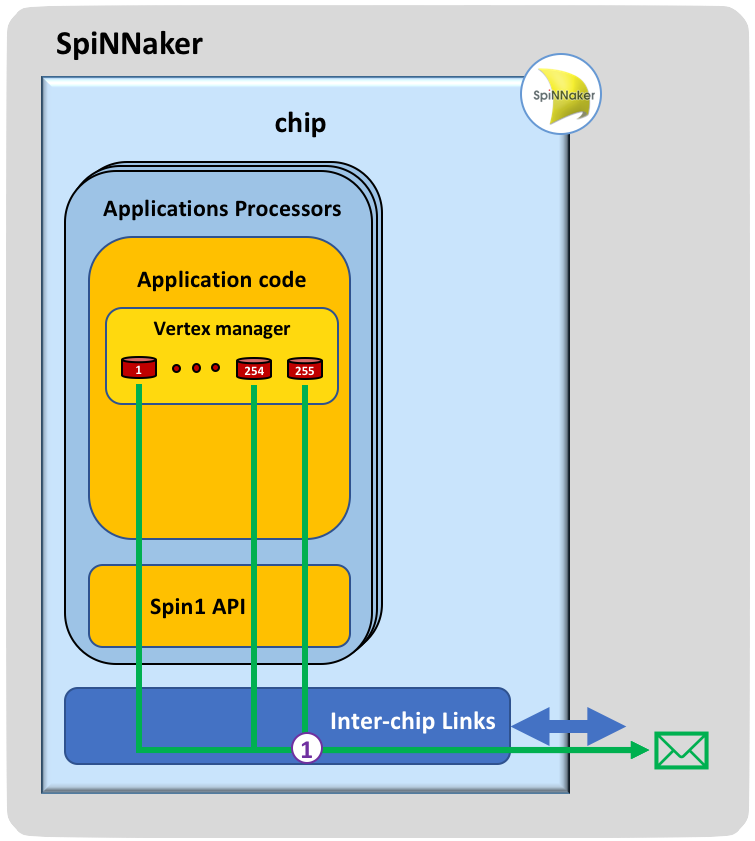
\includegraphics[width=0.82\hsize]{figures/impl-dataflow-out.png}
\caption{Data-flow of outbound messages in Page Rank under SpiNNaker.}
\label{fig:dataflow-out}
\end{figure}

The second step of the computation is more complex, and is related to the reception of inbound packets; see Fig.~\ref{fig:dataflow-in}. The steps described in this figure match the steps ordering described in the section \ref{sec:mplx} about multiplexing / demultiplexing. First, an incoming packet is buffered by the message processor (step 1) while its associated recipient records are loaded from SDRAM via a DMA transfer (step 2). Upon completion (step 3), the message dispatcher is called with the packet key / payload (green) and the loaded records (white) which are used to distribute the message to the specified Page Rank vertices (step 4).

\begin{figure}[hbtp]
\centering 
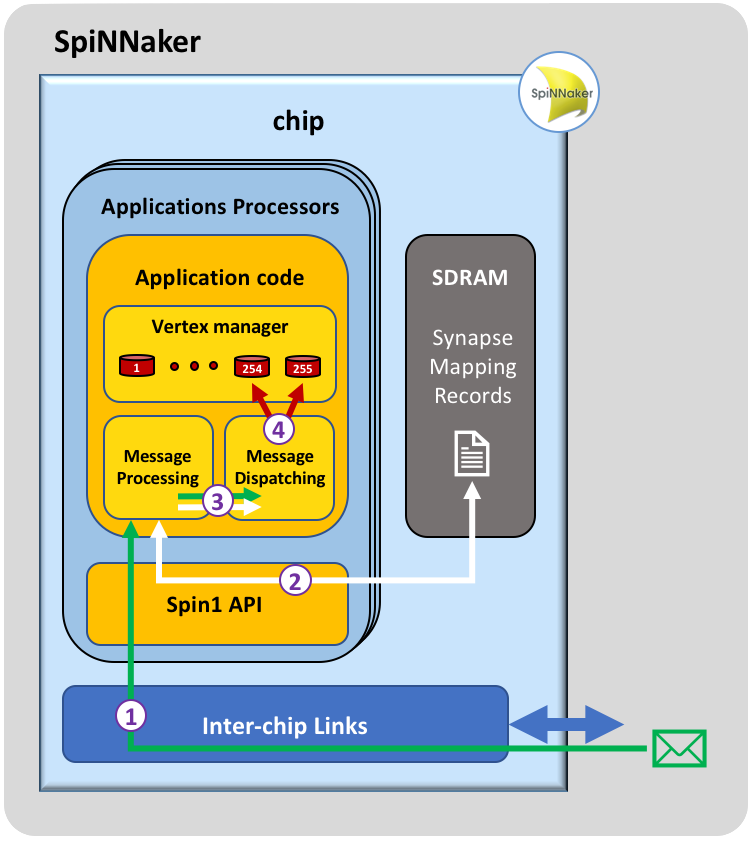
\includegraphics[width=0.9\hsize]{figures/impl-dataflow-in.png}
\caption{Data-flow of inbound messages in Page Rank under SpiNNaker.}
\label{fig:dataflow-in}
\end{figure}

Here again, this message processing strategy is derived from the original spike processing logic in \texttt{sPyNNaker}. Adapting an existing implementation that has proven its robustness through years of operations was an invaluable asset that made an efficient implementation of Page Rank possible. \\ 

Let us now review how iterations are synchronised in a world where there is no such thing as a synchronisation barrier. Indeed, neither the \texttt{Spin1} API nor the \texttt{SARK} library provide a way to globally synchronise all the cores across the system.

\paragraph{Locally synchronous, globally asynchronous}

In Page Rank, the results are computed iteratively one iteration after the other until a convergence point it reached. On a traditional single-threaded implementation, this is simply achieved by executing each iteration one after the other. On a traditional multi-threaded implementation, this is done by having a synchronisation barrier to wait for all workers to complete an iteration before moving to the next one. In SpiNNaker, there are no synchronisation barrier so it was decided to choose a locally synchronous, globally asynchronous approach. \\

Locally, each core waits for all its vertices to complete their iteration before moving to the next one, synchronously as a group. In practice, this is done by using the semaphore API provided by SARK, by having each vertex raise the semaphore at the beginning of the iteration and lower it when it has received all its expected packets. \\
 
Globally, cores are not synchronised and move at their own pace. In that setting, it is possible to have some packets that arrive early, sent by a core that is a few iterations ahead. To cope with this issue, all packets are tagged by the sender with an iteration number, and the receiver maintains distinct per-iteration buffers. Consequently, early packets are buffered until the core advances to the right iteration. Since a core only moves to the next iteration when \textit{all} its vertices have received \textit{all} their expected packets, these cross-core data flow dependencies should ensure (particularly on dense networks) that all cores progress approximately at the same pace. This reduces the need for an exhaustive list of buffers covering each iteration of the simulation; a cycling iteration time stamp of 4 iterations is sufficient in practice. \\

Overall, this implementation achieves good performance speed-ups, which are detailed in section \ref{sec:eval}, and allows Page Rank to scale at a minimal overhead.

\paragraph{Mitigating communication deadlocks}

Finally, a last corner case this implementation mitigates is communication deadlock; an example is visually described in Fig.~\ref{fig:pkt}. Indeed, if a packet is lost by the network, then its recipients could wait for its arrival indefinitely, blocking the entire computation. 

\begin{figure}[hbtp]
\centering 
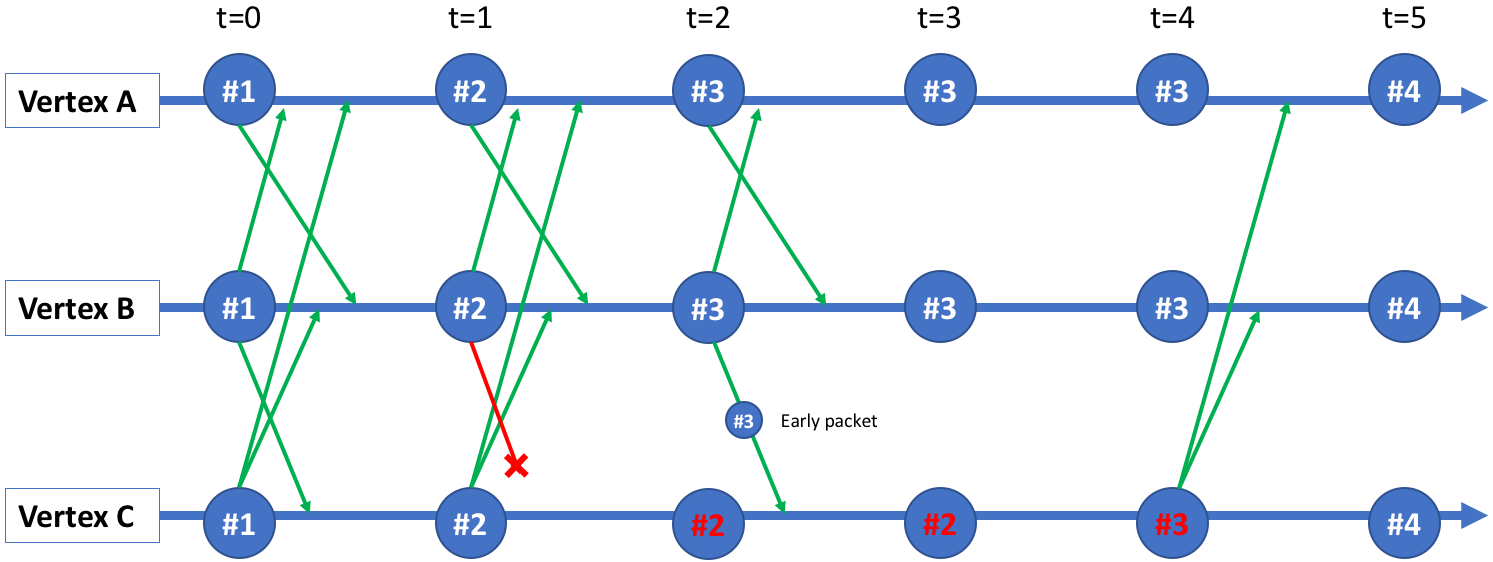
\includegraphics[width=1\hsize]{figures/packet_drop.png}
\caption{Data-flow diagram of packet loss and recovery in the globally asynchronous Page Rank model. This assumes each graph node (i.e. vertex) is on a different core.}
\label{fig:pkt}
\end{figure}

To cope with this issue, a time-out is included at the vertex manager level to force the next iteration if no change has occurred in the vertices' states for over 3 time steps. This threshold was chosen arbitrarily and requires tuning. Let us take the example from Fig.~\ref{fig:pkt}, which assumes all three graph vertices are on different SpiNNaker cores. We notice a packet is dropped during iteration at $t=1$ and causes a communication deadlock. Indeed, vertex C is still expecting a packet from iteration \#2 and vertices A et B wait for a packet from iteration \#3. We also notice an early packet reaches C, which does not cause a problem as the asynchronous model buffers early packets. At the third idle hardware time step at $t=4$, C detects it has deadlocked and forces the next iteration by resetting its state values to their content at the beginning of iteration \#2. It also sends its packets for iteration \#3 right away to A and B. At this point, all vertices have received the necessary packets for iteration \#3 and can move together to the next iteration. \\

However, this solution is quite fragile for two reasons: 

\begin{itemize}
\item The values computed are not correct anymore, since vertex C used old values from iteration \#2 for its iteration \#3. However, near-perfect solutions are still relevant for Page Rank so it is probably tolerable to have a minor level of noise in some outputs. Moveover, the simulation would then continue and converge, most likely erasing gradually the errors from the early stages.

\item Secondly, in the most likely case, A and B will have received updates at time $t=2$, like in this example, meaning their time-out would only occur at time $t=5$. This works correctly as the time-out will occur one step earlier on C, which will send its packet before iteration \#5 begins on A and B. However, if one of these vertices, say A, was only expecting an edge from C, than its time-out would have occurred at time $t=4$. This would have created a new deadlock phase centred around vertex A, and on larger graphs this could result into chains of time-outs that the simulation would not recover from.
\end{itemize}


Nonetheless, it can still allow the computation to recover from a few dropped packets, so it is kept for that purpose.
%EXPLAIN Sample 4 nodes exmaple


\subsection{Correctness considerations} \label{sec:resval}


To validate the correctness of the implementation above, a Python implementation was jointly used to verify the Page Rank results obtained on SpiNNaker. Comparing these results in that setting proved to be too imprecise, as SpiNNaker only supports fixed-point arithmetic operations while Python's floating-point representation is significantly more precise. Consequently, to ensure results would match to the exact bit, a binary fixed-point arithmetic library had to be used to re-implement the Python Page Rank implementation. \\

Additionally, since any remote automated testing (on a continuous integration platform for instance) is hardly doable without the physical board, we opted for local robustness testing. A performance testing script was made to generate arbitrary large graphs and run Page Rank computations on it, verifying each time the results with the Python implementation. This script was run before pushing any commit, and provided a local solution to have a minimal continuous assessment of the correctness of the implementation. \\

Finally, it is noteworthy to mention that \texttt{sPyNNaker} provides a way of collecting monitoring data from simulations. For instance, it counts the number of packets dropped by the network or by an overloaded core, which will be some valuable information for the evaluation section that follows.

%
%Can inspect the machine post-execution, so you know if you dropped some packets at some point. Guaranties you have the right results if no such error message
%
%Routing / chip, so if you make sure each Page Rank vertex is connected to at least another vertex on each of the 4 chips, you maximise the number of packets sent. Robustness tests (and everything in the evaluation section to follow) ran with 10 edges per vertex, ensuring an overwhelming probability that all nodes will be connected to another node of each chip.
%
%TODOs:
%	Exploited graph processing bencharmarks. However, they rely on generic graph processing algorithms whereas we can only run Page Rank for now.

\newpage
\section{Evaluation} \label{sec:eval}

The evaluation of the Page Rank simulation framework will comprise of two steps. First of all, we will give a brief overview of some benchmarking considerations - see section \ref{sec:bench}. Then, the first stage will focus on tuning the simulation parameters, which define the time allowance given to a Page Rank iteration to execute - see section \ref{sec:partun}. The second stage will demonstrate the performance achieved by SpiNNaker, first under varying placement conditions and then relative to a Python implementation of Page Rank - see section \ref{sec:perf}. \\

\subsection{Benchmarking  considerations} \label{sec:bench}

A key feature of these benchmarks is the parameters chosen to modulate the running time of a simulation. Considering a Page Rank graph that needs 10 iterations to converge, then two configuration parameters can influence its wall-clock time:

\begin{itemize}
\item \textbf{time\_step} (ms): hardware clock time between each timer tick. The bigger this time step the more time the core has between each timer tick.
\item \textbf{time\_scale\_factor} (unit-less): scales up the wall-clock execution time, by slowing down the notion of time on SpiNNaker by some factor. 
\end{itemize}

The table below illustrates the implications of different configurations of these parameters on the number of timer ticks and on the wall-clock running time.

\begin{center}
\begin{tabular}{ |c|c|c|c|c| }
 \hline
 sim. time & \texttt{time\_step} & \texttt{time\_scale\_factor} & \textbf{timer ticks} & \textbf{wall-clock time}  \\ 
 \hline
10 & 1 & 1 & 10 & \textbf{10} \\ 
10 & 2 & 1 & 5 & \textbf{10} \\ 
10 & 1 & 2 & 10 & \textbf{20} \\ 
 \hline
\end{tabular}
\end{center} 

This level of granularity between wall-clock execution time and SpiNNaker time was required by spiking neural networks simulations, but is not useful for Page Rank. Indeed, synapsic model can be time-based whereas Page Rank iterations do not have any such dependence. Consequently, we will be fixing the \texttt{time\_step} during this evaluation and varying the \texttt{time\_scale\_factor} to modulate the running time of Page Rank simulations. \\

Another relevant detail to note is that it seems hazardous to compare the raw running times of two machines of such different natures, such a a neuromorphic and a traditional personal computer. Therefore, all the comparisons we make will be based on arbitrary-unit running times and the point of interest will be the scaling trends of one machine versus the other. Other running times that do not involve cross-machine comparisons will be expressed in \texttt{time\_scale\_factor}, taking a constant simulation time throughout the entire evaluation. Hence, only the \texttt{time\_scale\_factor} defines the \textit{wall-clock} simulation time in that setting. The simulation time chosen is $2.5ms$, with the default \texttt{time\_step} of $0.1ms$ \cite{defts}, giving 25 timer ticks; hence up to 25 iterations for Page Rank. As we are not interested in Page Rank convergence here, we always run the 25 iterations of Page Rank to be able to compare the running times of different graphs. \\

Finally, let us recall several graph topology considerations to disambiguate any magical number used in this benchmark. To begin with, we use 10 edges for each vertex to maximise network usage (explained in \ref{sec:resval}). Additionally, it is important to remember that a SpiNNaker core manages 255 vertices by default, and each chip contains $15 \times 255 = 3,825$ vertices; the last application core being used to re-inject dropped packets. Also, the Spin3 (see Fig.~\ref{fig:spin3}), which we use for these tests, contains 4 SpiNNaker chips so the maximum number of vertices we can simulate is $4 \times 3,825 = 15,300$. \\

\subsection{Parameter tuning} \label{sec:partun}

When SpiNNaker is not allowed enough time to process packets during an each iteration, it starts dropping packets. This can occur at two different layers: (a) at the network layer with router buffers overflowing or (b) at the core level which is not allowed enough time to process the entire incoming workload.

\begin{figure}[!ht]
    \centering
    \begin{subfigure}[b]{0.5\textwidth}
        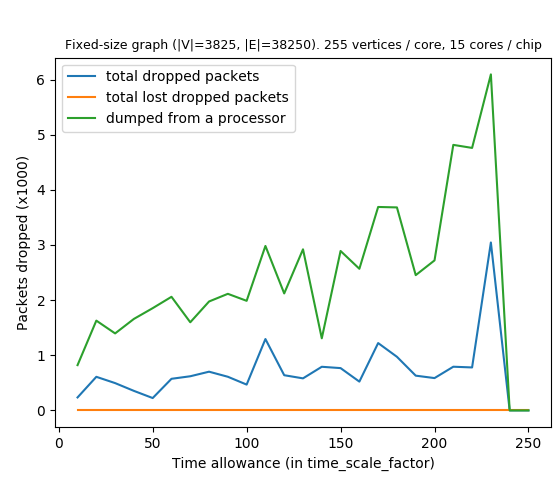
\includegraphics[width=\textwidth]{figures/packet_drop_vs_time_scale_factor-1.png}
        \caption{} \label{fig:graph11}
    \end{subfigure}%
    ~
    \begin{subfigure}[b]{0.5\textwidth}
        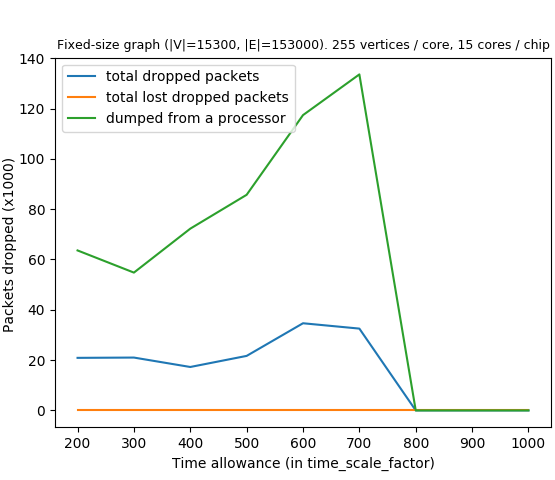
\includegraphics[width=\textwidth]{figures/packet_drop_vs_time_scale_factor-2.png}
        \caption{} \label{fig:graph12}
    \end{subfigure}
    \caption{Tuning hardware time step to avoid dropping packets}
    \label{fig:graph1}
\end{figure} 

In Fig.~\ref{fig:graph1}, we show an attempt to minimise the simulation running time while preventing packet drops for two sizes of graph. The first graph in Fig.~\ref{fig:graph11} fills an entire chip ($3,825$ vertices) and increases the \texttt{time\_scale\_factor} iteratively, while the second graph in Fig.~\ref{fig:graph12} fills all four chips of the board ($15,300$ vertices). For the first graph, we can note that $\texttt{time\_scale\_factor} = 230$ is the value from which Page Rank has enough time to be computed successfully, while this number is below $800$ for a bigger graph. Already, we can see that for 4 times the graph size (4 chips vs. 1 chip), the running time is only multiplied by $800/230 = 3.5$. This is a positive scaling result for an algorithm, Page Rank, that has a complexity of $O(|V|+|E|)$ that is linear in the sum of vertices and edges. \\

Maybe surprisingly, we note as a general trend that the more time we allow for execution, the more packets get dropped. This is due to the number of packets sent also increasing with \texttt{time\_scale\_factor}. Indeed, less time meant cores got interrupted before even sending all of their packets. \\

A second takeaway from these graphs is certainly the comparison between the two sources of bottlenecks: network usage \& core processing. On both graph sizes, the number of packets dropped by cores (green curve) increases faster than the number of packets dropped by the network (blue curve). Moreover, absolutely all packets dropped by the network get successfully re-injected in the network, as indicated by the flat orange curve at $y=0$. This indicates the cores are the main bottleneck of the computation. To keep the same processing capabilities in terms of graph size, the Page Rank framework code running on the cores could be made more efficient. However, the existing implementation, which is based on the partly-optimised neuron implementation of \texttt{sPyNNaker}, is already relatively optimised and might not have a lot of speed-up potential left to exploit. Another option is to reduce the number of vertices that a single core manages. The latter is an option that will be covered in the next section \ref{sec:perf}, but we can already note its main drawback is the reduced capability in terms of graph size input. Indeed, if $15,300$ vertices already filled up the entire board, then dividing by half the number of vertices per core would also divide by half that maximum capacity of $15,300$ down to $7,650$ vertices. \\

This now leads us to the second stage of this evaluation, where we will be covering the performance achieved by this project after porting Page Rank to SpiNNaker. \\

\subsection{Performance measure} \label{sec:perf}

\subsubsection{Resources vs. performance trade-off}

This first preliminary benchmark is interested in the performance trade-off mentioned earlier, where running time and resource utilisation oppose each other. Indeed, less vertices managed by core means poorer resource utilisation, so let us see to what extent it gives better running times that would justify compromising on resources - see Fig.~\ref{fig:graph2}.

\begin{figure}[!ht]
    \centering
    \begin{subfigure}[b]{0.5\textwidth}
        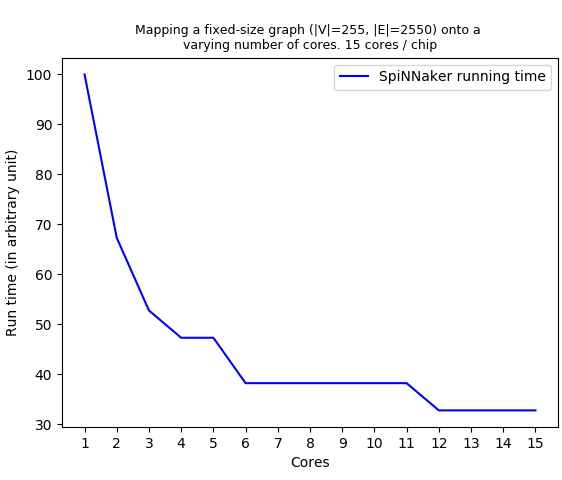
\includegraphics[width=\textwidth]{figures/atoms_per_core_vs_running_time-1.png}
        \caption{} \label{fig:graph21}
    \end{subfigure}%
    ~
    \begin{subfigure}[b]{0.5\textwidth}
        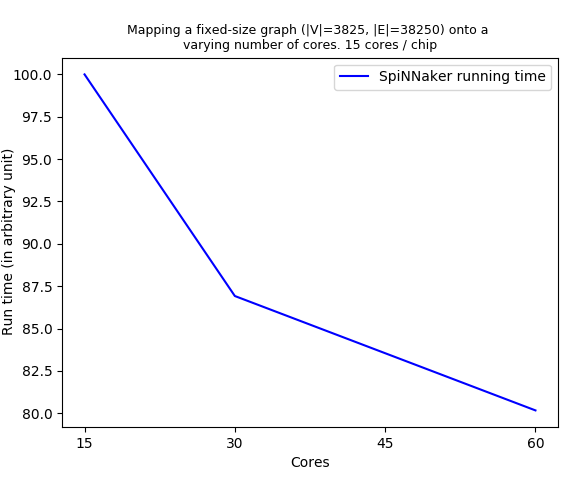
\includegraphics[width=\textwidth]{figures/atoms_per_core_vs_running_time-2.png}
        \caption{} \label{fig:graph22}
    \end{subfigure}
    \caption{Tuning number of Page Rank vertices managed by a single core}
    \label{fig:graph2}
\end{figure} 

In Fig.~\ref{fig:graph2}, the first graph \ref{fig:graph21} takes a fixed-size graph that fits on a single core, which is then partitioned into a varying number of cores. In practice, this is done by setting a constant at runtime that defines how many vertices of the graph should be mapped by \texttt{PACMAN} to a single core. Here, it is quite clear that the greater the number of nodes for the same graph, the better the running time is. However, this trend seems to tapper off from 6 cores onwards. For example, splitting this graph between 4 cores, managing $255 / 4 \approx 64$ vertices each, reduces the running time by more than half. \\

However on the second graph \ref{fig:graph22}, a similar trend is observed but to a lesser extent. Indeed, when quadrupling the number of cores used for the simulation (from 15 to 60), the running time is only reduced by $-20\%$ (from $100$ down to $80$) whereas it decreased by over $-50\%$ in the first case. This is due to: (a) the network overhead of a larger graph and (b), the added cost of chip-to-chip communication, which was not present in the previous case where all cores were on the same chip. \\

All in all, this experiment encourages SpiNNaker users to divide their graphs so that they are mapped to as many cores as possible and make full use of the hardware capabilities of the machine. This also shows this network load could be reduces by a clever partitioning of graph that minimises the chip-to-chip communication overhead.

\subsubsection{Performance at scale}

Finally, this last experiment is the most important one as is compares the scaling potential of Page Rank on SpiNNaker versus an implementation running on a traditional PC. For the Python implementation, we use an adapted version of the Page Rank algorithm from the \texttt{networkx} \cite{networkx} network manipulation library. The trace of running times of both machines are normalised relative to their first value, so that both scaling curves have the same starting point - see Fig.~\ref{fig:graph3}. These arbitrary units make the Core Processing Unit (CPU) model of the PC used irrelevant, as the scaling curve will have the same shape no matter how fast it runs on a given CPU.

\begin{figure}[!ht]
    \centering
    \begin{subfigure}[b]{0.5\textwidth}
        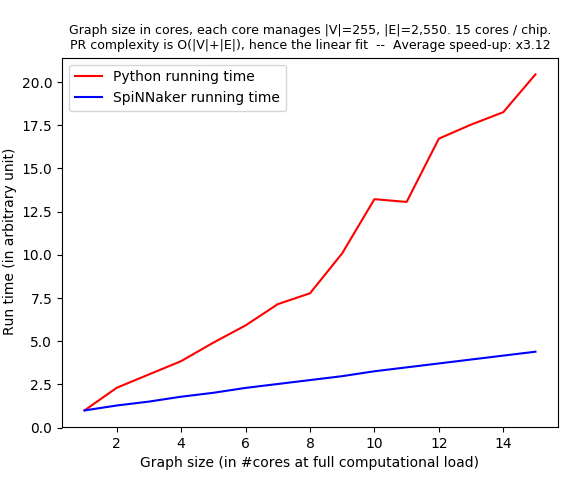
\includegraphics[width=\textwidth]{figures/graph_size_vs_running_time-1.png}
        \caption{} \label{fig:graph31}
    \end{subfigure}%
    ~
    \begin{subfigure}[b]{0.5\textwidth}
        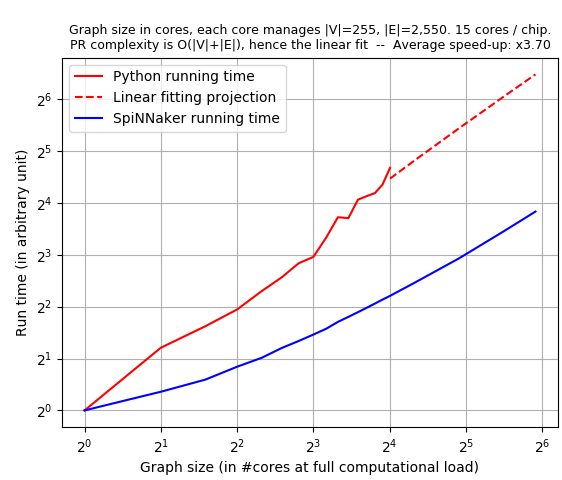
\includegraphics[width=\textwidth]{figures/graph_size_vs_running_time-2.png}
        \caption{} \label{fig:graph32}
    \end{subfigure}
    \caption{Page Rank (PR) scalability of Python vs. SpiNNaker}
    \label{fig:graph3}
\end{figure} 

First of all, we observe on both graphs that the scaling curves are approximately linear, which is consistent with the complexity $O(|V|+|E|)$ of Page Rank that remains unchanged. In Fig.~\ref{fig:graph31}, we see how both implementations scale on a graph that gradually fits up to an entire chip, that is $3,825$ vertices and ten times more edges. We also observe SpiNNaker brings a significant speed up in terms of scaling trend, averaged at a factor of x$3.12$ (see figure title). Likewise in Fig.~\ref{fig:graph32}, SpiNNaker clearly outperforms the traditional PC at a comparable speed-up factor of $3.70$ when scaling to larger graph sizes. Last but not least, for the last data point of the graph at $x=60$, the speed-up obtained is around $5$ while it is smaller for the first data points. This reveals that the scaling potential of SpiNNaker is not constant compared to the PC, but rather that it increases with larger graph sizes which is another positive contribution. \\

Overall, this evaluation confirms Page Rank on SpiNNaker has a significant scaling potential compared to a standard implementation running on a PC. It also shed light on the bottleneck of the current implementation, which is the heavy workload processed by cores. This leaves some further scaling opportunities for a follow-up project that would optimise the current Page Rank framework and potentially generalise it to other graph-based algorithms with comparable data flows. Lastly, it is interesting to see how efficient packet re-injection is. A better implementation on the processing cores that would push the bottleneck to the network could always lower the threshold from 0 packet dropped to 0 lost dropped packet (see Fig.~\ref{fig:graph1}). \\

\textit{Nota bene}: all the scripts used to run this benchmark can be found in the examples folder of the project folder, under \texttt{python/page\_rank/examples/plot\_*.py}.

\subsection{Limitations} \label{sec:lim}

Nonetheless, the implementation also has its limits which might discourage real-life graph processing applications of SpiNNaker. Firstly, the input size accepted by this implementation is limited by the hardware used. As show in the results above, the largest graph that can run on the Spin3 chip contained $15,300$ vertices. Even when using the biggest version of the machine, we would still not be able to process the largest graphs from Google or Facebook. Indeed, that machine has $1,036,800 cores$, of which only $15/18$ run the application code of the simulation, meaning the maximum number of vertices we could accept would be: $1,036,800 \times 15 \ 18 \times 255 = 220M$. With such capacities, SpiNNaker cannot compete with very large scale graph processing tools. \\

Moreover, the start-up time of simulations was not taken into account here. Indeed, the vast majority of the time is spent pre-processing the graph, the main bottleneck being the construction of the data specification which is loaded on SpiNNaker. Only long running algorithms would justify the upfront cost required by this pre-processing stage, and Page Rank usually converges in a few hundreds of iterations, which get computed relatively fast. Large graph inputs should be benchmarked to confirm if the start-up cost can be compensated by the running time speed-up on SpiNNaker. \\

This perfectly introduces one of the problems of this evaluation, which is that it only ran on small machine. Although the results are encouraging for larger graphs, only a proper testing phase on a bigger machine could confirm the true scalability potential of this Page Rank simulation framework. This would also allow for the asynchronous model to be tested, as it is more likely iterations will get out of synchronisation on a bigger input graph mapped to a large number of cores.

\newpage
\section{Conclusion}

Overall, this project has been successful in demonstrating the scaling potential of SpiNNaker on a new algorithm, specifically Page Rank here, that had never been implemented on the machine before. This unveils new scaling opportunities for a whole problem class of graph-based algorithms with similar data-flow patterns, which are also expected to yield equivalent speed-ups. These algorithms are characterised by a large amount of state that needs to be maintained and shared throughout the computation. On a distributed system running on large graphs, exchanging that state between workers can rapidly become the bottleneck. The true edge of SpiNNaker is its low-latency interconnect between computational chips, that outperforms the standard end-to-end latency between servers of a cluster. We can only hope this proof of concept could motivate new research projects to investigate further how SpiNNaker could speed up graph-based algorithms. Indeed, some challenges remain unsolved after this project, such as limitations regarding the input graph size or the start-up cost of a simulation. \\

The second contribution is related to tooling and supports the speed-up claim of this project. The Page Rank simulation framework built demonstrates how the paradigm of spiking neural networks can be mapped to Page Rank. However, this implementation is far from being a final solution for porting Page Rank to SpiNNaker and there is still plenty of opportunities for improvement. A follow-up project could work on these improvements, such as random back-off delays interleaving sent packets during network congestion or full asynchronous control flow by removing the main timer tick. Additionally, the framework could be made more generic to easily accommodate new graph-based algorithms, just as the research team from Markov Chain Monte Carlo Inference designed a generic framework to support Markov Chains on SpiNNaker \cite{markov-on-spinn}. \\


\footnotetext{Word count: 19,448 words} 




\newpage
\appendix
\section{Appendix - Simple sPyNNaker8 full simulation code} \label{app:a}

The following code was adapted from \cite{pynnsim}.

\begin{minted}{python}
import spynnaker8 as sim
import pyNN.utility.plotting as plot
import matplotlib.pyplot as plt


# Setup SpiNNaker with for 1 microsec time steps
sim.setup(timestep=1.0)

# Define a population of 1 neuron that will spike once at time t=0
pIn = sim.Population(1, sim.SpikeSourceArray(spike_times=[0]), label="input")
# Define a population of 1 neuron with neuron model `IF_curr_exp'
pOut = sim.Population(1, sim.IF_curr_exp(), label="output")
# Define a synapse link pIn -> pOut with synapse model `StaticSynapse'
sim.Projection(pIn, pOut, sim.OneToOneConnector(),
                     synapse_type=sim.StaticSynapse(weight=5, delay=1))

# Set spikes and voltage to be recorded at each time step
pOut.record(["spikes", "v"])

# Starts the simulation
simtime = 10  # ms
sim.run(simtime)

# Collect recorded data
neo = pOut.get_data(variables=["spikes", "v"])
spikes = neo.segments[0].spiketrains
v = neo.segments[0].filter(name='v')[0]
sim.end()

# Display graphs
plot.Figure(
    # plot voltage for first ([0]) neuron
    plot.Panel(v, ylabel="Membrane potential (mV)", data_labels=[pOut.label],
               yticks=True, xlim=(0, simtime)),
    # plot spikes (or in this case spike)
    plot.Panel(spikes, yticks=True, markersize=5, xlim=(0, simtime)),
    title="Simple Example",
    annotations="Simulated with {}".format(sim.name())
)
plt.show()
\end{minted}

\newpage
%\bibliographystyle{alpha}
%\bibliographystyle{ieeetr}
\bibliographystyle{IEEEtran}
\bibliography{bibs/references}

\end{document}